%% ISA Transactions manuscript -- Elsevier elsarticle template
%% Compile: pdflatex main; pdflatex main  (bibliography is inline, no BibTeX needed)
\documentclass[preprint,12pt,authoryear=false]{elsarticle}
\usepackage[T1]{fontenc}
\usepackage[utf8]{inputenc}
\usepackage{lmodern}
\usepackage{amsmath,amssymb,mathtools,bm}
\usepackage{booktabs,array,multirow,graphicx,siunitx}
\usepackage{microtype,xcolor}
\usepackage[colorlinks=true,urlcolor=blue!50!black,linkcolor=blue!50!black,citecolor=blue!50!black]{hyperref}
\usepackage{lineno}
\usepackage{amsthm}
\usepackage{algorithm}
\usepackage{algpseudocode}
\theoremstyle{remark}\newtheorem{remark}{Remark}
\theoremstyle{plain}\newtheorem{proposition}{Proposition}\newtheorem{lemma}{Lemma}
\theoremstyle{definition}\newtheorem{assumption}{Assumption}

\newcommand{\tmax}{\tau_{\max}}
\newcommand{\Nm}{\,\mathrm{N\,m}}
\newcommand{\todo}[1]{\textcolor{red}{[TODO: #1]}}
\journal{ISA Transactions}

\begin{document}
\begin{frontmatter}

\title{Fault-Tolerant Roll Stabilization of a CMG-Actuated Motorcycle:\\
Robust EKF--MPC versus Distilled Neural MPC and Residual Reinforcement Learning}

\author[inst1]{S. M. Razavi-Nabavi}
\ead{sm.razavinabavi@ut.ac.ir}

\author[inst1]{M. Ayati\corref{cor1}}
\ead{m.ayati@ut.ac.ir}

\author[inst1]{Taraneh Mahdibehesht}
\ead{sm.razavinabavi@ut.ac.ir}

\cortext[cor1]{Corresponding author}
\address[inst1]{Advanced Instrumentation Laboratory, School of Mechanical Engineering, University of Tehran, Tehran, Iran}

\begin{abstract}
Fault-tolerant roll stabilization of a simulated motorcycle actuated by two control-moment gyroscopes (CMGs) is studied under roll-measurement faults. Four controller families are compared on matched seeds and initial conditions: a neural network distilled from a constrained model predictive controller (MPC), a Pure soft actor--critic (SAC) policy outputting torque directly, a bounded residual SAC correction to the neural MPC, and online MPC supplied with a robust extended Kalman filter (EKF). With horizon $N=20$, EKF--MPC completes 82.0\% of five-second episodes under 50\% roll-measurement dropout and 57.0\% under 20-step intermittent corruption, versus 60.7\% and 32.3\% for residual SAC. The same online MPC without the estimator completes 1.0\% of the 50\%-dropout episodes (1.7\% with a gate-only EKF), so the benefit stems from the estimator's stale-data and covariance-recovery logic rather than from online optimization. When all controllers receive the same robust EKF output, the distilled neural MPC reaches 82.3\% and 56.7\% (85.7\% five-scenario mean), identical to EKF--MPC, and residual SAC 81.0\% and 55.6\%; the advantage seen on raw measurements is thus carried by the information pathway. This conclusion is conditional on an exact filter model, however: in a supplementary stress test combining sensor noise (matched to the filter's noise model) with a 20\% rotor-inertia reduction, EKF--MPC completion falls from 100\% to 84.0\% (4{,}173 roll-channel innovation rejections, roll-estimation error 0.077\,rad), whereas residual SAC on raw measurements completes 99.7\% and the neural and online MPC 97.3\%. On the tested CPU, the distilled network matches the teacher's healthy-plant completion rate at roughly $1/181$ of the command-computation time, but remains sensitive to rotor-inertia reduction. Cross-simulator evaluation in MuJoCo shows that the omitted gimbal-angle dependence of CMG torque, and the presence of a gimbal stop or torque supervisor, strongly affect transferred performance (residual SAC: 75.3\% to 3.1\% unmodified; 40.0\% and 43.6\% with stop or supervisor), which yields concrete design requirements for future hardware validation. A conditional boundedness analysis, including a lemma on the gated update, states the properties that a closed-loop certificate for the learned stack would have to establish.
\end{abstract}

\begin{keyword}
motorcycle roll stabilization \sep control-moment gyroscope \sep fault-tolerant control \sep residual reinforcement learning \sep soft actor--critic \sep extended Kalman filter \sep model predictive control \sep sim-to-sim transfer
\end{keyword}
\end{frontmatter}

\linenumbers

%==============================================================
\section{Introduction}
Maintaining the roll equilibrium of an inherently unstable motorcycle requires rapid compensation of gravity-induced tipping and gyroscopic interactions. A pair of control-moment gyroscopes (CMGs) can generate roll-control authority by changing the direction of rotor angular momentum. Constrained model predictive control (MPC) is attractive because actuator torque and gimbal angle and rate limits can be handled in a single optimization. However, repeated finite-horizon optimization may be expensive, and performance can deteriorate when roll-angle and roll-rate measurements become unreliable.

Two complementary approaches are considered. In the first, a feed-forward neural network imitates the first action of an offline MPC teacher, and a residual SAC policy learns an additive, bounded correction (Fig.~\ref{fig:arch}), following the residual reinforcement-learning paradigm \cite{johannink2019residual} with SAC as an off-policy maximum-entropy method \cite{haarnoja2018soft,haarnoja2018softapps}; learned and differentiable MPC \cite{amos2018differentiable} is closely related. In the second, the constrained MPC remains online, but its state information is provided by an EKF \cite{kalman1960new} supplemented by innovation gating, stale-signal detection and covariance recovery. The first approach addresses online inference cost and behavioral correction; the second addresses faulty feedback explicitly through estimation and optimization. They should not be treated as interchangeable implementations.

The study is organized around four questions that single-controller demonstrations leave open:
\begin{itemize}
\item \textbf{Q1} How much closed-loop performance is lost, and how much computation is saved, when online MPC is replaced with a distilled neural network?
\item \textbf{Q2} Does a bounded SAC residual improve the distilled baseline, and under which fault and model-mismatch conditions?
\item \textbf{Q3} When roll measurements are unreliable, how does estimator-aided online MPC compare with learned policies that directly receive corrupted measurements?
\item \textbf{Q4} Do policies trained on a reduced-order model retain their performance on a higher-fidelity CMG simulation without retraining?
\end{itemize}
The contributions are:
\begin{enumerate}
\item a common reduced-order motorcycle--CMG model and a matched roll-measurement fault evaluation protocol;
\item a comparison of neural MPC, Pure SAC, residual SAC and EKF--MPC on matched fault realizations, including matched-information runs in which every controller receives the output of the same robust EKF (Section~\ref{sec:ablation});
\item a prediction-horizon study of EKF--MPC (completion, survivor-conditioned tracking, effort, solver timing and solver-status accounting) from a single complete run with frozen settings, together with an estimator ablation of the online MPC and a supplementary stress test of the estimator under sensor noise and rotor-inertia mismatch (Section~\ref{sec:noisemis});
\item an MPC-to-network distillation assessment using held-out torque error, paired closed-loop completion and measured command-computation time (Section~\ref{sec:nn});
\item a held-out cross-simulator assessment of frozen policies on a higher-fidelity, gimbal-angle-dependent MuJoCo model \cite{todorov2012mujoco}, separating unmodified transfer from physical and supervisory interventions.
\end{enumerate}
The contribution is an integrated fault-tolerant roll-stabilization framework (robust EKF, constrained MPC, its distilled network and a bounded residual policy, built from established components), together with a matched-information analysis of where fault tolerance originates and a cross-simulator analysis of how the resulting behavior transfers to a higher-fidelity CMG model. The complementary 34-scenario benchmark (Section~\ref{sec:34}) is reported separately and is not pooled with the focused cohort. The study is a reproducible simulation comparison, not evidence of deployment-ready functional safety; the MuJoCo model is not a complete contact-rich riding-motorcycle model.

%==============================================================
\section{Related work}
\label{sec:related_work}

\subsection{CMG-based stabilization and single-track vehicle dynamics}
Control-moment gyroscopes (CMGs) are momentum-exchange actuators that are widely used for spacecraft attitude control~\cite{wie2001singularity,schaub1998cmg}. They have also been applied to two-wheeled vehicles, where a gyroscopic torque can balance the vehicle when speed is too low for steering to supply a sufficient restoring moment~\cite{beznos1998control,yetkin2014gyro,tofigh2021fractional,zheng2022dynamic}. Beznos et al.~\cite{beznos1998control} described a bicycle with a stabilization unit of two coupled gyroscopes spinning in opposite directions; the precession torque counteracts the gravity torque, and the bicycle moved autonomously along straight and curved paths. Yetkin et al.~\cite{yetkin2014gyro} designed a first-order sliding-mode controller for a single CMG that stabilizes a bicycle at zero forward velocity and compared it with a PID controller. Tofigh et al.~\cite{tofigh2021fractional} proposed a twin-flywheel gyrostabilizer that can provide a desired gyroscopic roll moment, derived a Newton--Euler bicycle model that includes the actuator dynamics, and designed a robust fractional-order sliding-mode controller for tracking under roll disturbance; the evaluation is in simulation with experimentally measured bicycle parameters. Zheng et al.~\cite{zheng2022dynamic} built a multibody model of an unmanned motorcycle (Lagrange equations of the first kind), derived a simplified model for control design, and showed in simulation that a combined steering and double-CMG controller outperforms a steering controller and an inverted-pendulum-based controller. To our knowledge, none of these studies treats corrupted roll measurements; they address nominal balance or disturbance rejection.

A central kinematic issue in CMG systems is \emph{gimbal singularity}, where the gimbal configuration cannot produce torque along the commanded direction~\cite{wie2001singularity,takada2010control}. Aerospace work addresses it with singularity-robust inverse steering logic~\cite{wie2001singularity}, with cost-function-based avoidance~\cite{takada2010control}, and with global steering by heuristic search~\cite{papakonstantinou2021global}; a feedback law for variable-speed CMGs is given in~\cite{schaub1998cmg}. Vehicle studies typically design controllers on simplified models~\cite{zheng2022dynamic}. As Section~\ref{sec:cross} shows, a policy trained on a reduced-order model that omits the gimbal-angle dependence of CMG torque degrades strongly when transferred to a higher-fidelity model that includes it.

\subsection{Model predictive control and neural distillation}
Model predictive control (MPC) handles state, torque and gimbal constraints in one optimization~\cite{rawlings2017model}, and operator-splitting solvers such as OSQP~\cite{stellato2020osqp} make the underlying quadratic programs (QPs) fast. A QP must nevertheless be solved at every step (here at \SI{100}{\hertz}, Table~\ref{tab:par}), which can be demanding on embedded hardware.

Approximating the MPC law offline by a neural network is an established remedy. Parisini and Zoppoli~\cite{parisini1995neural} approximated a nonlinear receding-horizon regulator for discrete-time systems with state and control constraints by a multilayer feedforward network computed off-line, and established bounds on the approximation. Karg and Lucia~\cite{karg2020efficient} showed that ReLU networks can exactly represent the piecewise-affine MPC law of linear systems, gave bounds on the required depth and width, and suggested ways to correct or quantify the approximation error. Hertneck et al.~\cite{hertneck2018learning} learn an approximate MPC with closed-loop guarantees. Chen et al.~\cite{chen2022large} combine an offline-trained network, trained with a primal--dual loss, with an online primal active-set solver that provides recursive feasibility and asymptotic stability, and report a $2\times$ reduction in online inference time against the best method of their benchmark. Differentiable MPC~\cite{amos2018differentiable} instead embeds the optimization in a learning pipeline. Our distillation is empirical behavioral cloning of the first MPC action and carries no such guarantee; we therefore report held-out error, paired closed-loop behavior and timing (Section~\ref{sec:nn}).

\subsection{Residual reinforcement learning and safety filters}
Residual reinforcement learning adds a learned correction to a conventional controller. Johannink et al.~\cite{johannink2019residual} combined a hand-designed controller with a learned residual for robotic manipulation under contact, and Silver et al.~\cite{silver2018residual} learn a residual on top of a fixed, imperfect controller; both report that starting from the baseline makes learning more data-efficient than learning from scratch. We learn the residual with Soft Actor-Critic (SAC)~\cite{haarnoja2018soft,haarnoja2018softapps}, an off-policy maximum-entropy actor--critic method.

A different route to safety is the control barrier function (CBF)~\cite{ames2019control}, which enforces forward invariance of a safe set through a QP, and its high-order extension (HOCBF) for constraints of arbitrary relative degree~\cite{xiao2022high}. Here the residual is clipped to a norm bound $\tau^{\rm res}_{\max}$, so the applied torque differs from the clipped baseline torque by a bounded amount, and Section~\ref{sec:bound} derives a conditional ultimate-boundedness result (Proposition~\ref{prop:ub}) that assumes input-to-state stability of the baseline loop.

\subsection{Fault-tolerant control and robust Kalman state estimation}
Sensor faults threaten closed-loop stability, and fault-tolerant control (FTC) combines fault detection and isolation with state estimation~\cite{blanke2016diagnosis,isermann2011fault,patton2000fault}. We organize the work closest to our estimator--controller design along five topics.

\paragraph{Observer-based sensor-fault handling.}
A common model-based approach is to estimate the fault or the state from healthy information and to feed the controller a fault-free estimate. Tan and Edwards~\cite{tan2002sliding} used sliding-mode observers to detect and reconstruct sensor faults; Du and Mhaskar~\cite{du2014isolation} isolate a faulty sensor with a bank of observers and then use the estimate from the healthy sensors in closed loop; Ait~Ladel et al.~\cite{ailadel2021integrated} estimate sensor faults and design observer-based control for switched systems through a separation principle solved by linear matrix inequalities; and Sun et al.~\cite{sun2025adaptive} fuse redundant sensors with weights that suppress faulty ones inside an adaptive output-feedback controller. Work from the University of Tehran follows the same line: Ayati and Nikbakht~\cite{ayati2016pmsm} use two sliding-mode observers as virtual sensors that replace faulty measurements of a permanent-magnet synchronous motor once a fault is detected, Ayati and Salmasi~\cite{ayati2015fault} detect and approximate faults of linear impulsive systems with a sliding-mode observer, and Rahnavard et al.~\cite{rahnavard2017sliding,rahnavard2019finite} reconstruct actuator faults and states of a wind-turbine benchmark. Our EKF--MPC shares the principle of replacing a rejected measurement by a model-based estimate, but uses a Kalman filter with innovation gating instead of fault-reconstructing observers, and the controller is an online constrained MPC.

\paragraph{Robust extended Kalman filtering.}
The Kalman filter~\cite{kalman1960new} is the standard estimator under Gaussian noise, and several robust EKF designs address its sensitivity. Einicke and White~\cite{einicke1999robust} designed a discrete-time EKF with $H_\infty$ methods to limit the effect of linearization errors. Fang et al.~\cite{fang2022robust} made the EKF robust against measurement outliers of various magnitudes, types and durations through an innovation-saturation mechanism with adaptive bounds, without requiring measurement redundancy, and characterized the stability of the approach for linear systems. These designs bound the influence of an abnormal innovation. Our filter instead rejects a roll sample through a hard $\chi^2$ gate, and it adds a stale-data indicator and a covariance-recovery rule for long outages (Section~\ref{sec:ekf}).

\paragraph{Innovation-based fault detection.}
Monitoring the innovation sequence of a Kalman filter with statistical tests is a classical route to fault detection and diagnosis~\cite{mehra1971innovations}; Willsky~\cite{willsky1976survey} surveys design methods for detecting abrupt changes in stochastic dynamic systems. The validation gate, a Mahalanobis-distance test with a $\chi^2$ threshold, is standard in tracking~\cite{barshalom2001estimation}, and Song et al.~\cite{song2024innovation} apply a Chi-square test on the innovations of a GPS/SINS navigation filter to detect faults and to degrade or isolate abnormal innovations. Our gate uses the same statistic on the two-dimensional roll innovation. Its limits for an open-loop unstable plant are examined in Lemma~\ref{lem:gate}: with the gate alone, a long run of rejected samples leaves the filter either rejecting valid data or, after unbounded covariance growth, trusting corrupted samples.

\paragraph{Multiple sensor faults.}
Pazera et al.~\cite{pazera2018robust} estimate all sensor faults of a nonlinear system with a single observer and use the fault-free state for control, with a separation principle that allows the estimator and the controller to be designed separately; they report an experimental study on a twin-rotor system. Sun et al.~\cite{sun2025adaptive} and Du and Mhaskar~\cite{du2014isolation} likewise address plants with several sensors, of which some may fail. In our study the injected faults (dropout, burst corruption, stuck values) affect only the roll-angle and roll-rate channels, while the gimbal measurements remain healthy; simultaneous faults on several channels are outside our evaluation (Section~\ref{sec:limits}).

\paragraph{State estimation under intermittent measurements.}
Sinopoli et al.~\cite{sinopoli2004kalman} modeled the arrival of observations as a random process and showed that the error covariance of the Kalman filter has a critical arrival rate beyond which it becomes unbounded; adaptive estimation of noise covariances goes back to Mehra~\cite{mehra1970identification}. A long roll dropout in an open-loop unstable plant is the corresponding situation here. The inflation-and-capping step of Section~\ref{sec:ekf} is an engineering recovery rule that keeps the filter receptive when the sensor returns; it is not derived from that analysis, and we state its guarantee only through Lemma~\ref{lem:gate}.

\paragraph{Fault accommodation in vehicle control.}
For road vehicles, Zarringhalam et al.~\cite{zarringhalam2013optimal} studied the observability of yaw, roll and lateral states of a 3-DOF vehicle model for different sensor configurations and developed a fault-tolerant adaptive estimator that mitigates the effect of sensor failures, evaluated numerically and in CarSim. Tao et al.~\cite{tao2024simultaneous} combine a dynamic observer with a neural network to estimate the state and sensor faults of an autonomous vehicle under modeling uncertainty. These works concern estimation of vehicle states or faults; to our reading they do not compare constrained, distilled and reinforcement-learning controllers under the same sensor faults, which is what this paper does for a CMG-balanced motorcycle.

\subsection{Sim-to-sim and sim-to-real transfer gaps}
Domain randomization~\cite{tobin2017domain} and dynamics randomization~\cite{peng2018sim} expose policies to a distribution of parameters, which addresses parametric mismatch but not a structural omission in the training model. Henderson et al.~\cite{henderson2018deep} showed that deep-RL results depend strongly on seeds, implementation details and reporting, which motivates our matched-seed, paired protocol. Our transfer study isolates one such structural omission, the gimbal-angle dependence of CMG torque: in the higher-fidelity MuJoCo model~\cite{todorov2012mujoco}, which is not a complete contact-rich riding-motorcycle model, learned policies park the gimbals where the available roll authority vanishes (Section~\ref{sec:mech}).

\subsection{Literature gap and research positioning}
Table~\ref{tab:literature_comparison} places this study among the works reviewed above. Each ingredient of our framework is established on its own: CMG balance control, neural approximation of MPC, residual reinforcement learning, and Kalman-filter-based handling of sensor faults. We therefore do not claim that no related work exists. The gap we address is narrower: among the works reviewed in this section, we found none that compares learned and online-optimized controllers for a CMG-balanced single-track vehicle under roll-measurement faults within one controlled protocol. Our study differs from the reviewed works in three documented respects.
\begin{enumerate}
\item[(i)] \textbf{Matched fault seeds.} Neural MPC, Pure SAC, residual SAC and EKF--MPC are evaluated on identical fault realizations, initial conditions, references and noise, and the survival and tracking contrasts are paired and use hierarchical bootstrap with Holm correction (Section~\ref{sec:results}). The reviewed CMG-vehicle studies~\cite{beznos1998control,yetkin2014gyro,tofigh2021fractional,zheng2022dynamic} treat nominal balance or roll disturbance and do not inject measurement faults, and the reviewed estimation and fault-tolerant control studies~\cite{fang2022robust,pazera2018robust,zarringhalam2013optimal} do not involve learned controllers.
\item[(ii)] \textbf{Matched information.} To separate the benefit of online optimization from that of the estimation pathway, every controller is also run with the output of the same robust EKF (Section~\ref{sec:ablation}, Table~\ref{tab:match}), in addition to raw measurements. In our results the distilled neural MPC fails on raw corrupted measurements but matches EKF--MPC when it receives the EKF output.
\item[(iii)] \textbf{Cross-simulator evaluation.} Frozen learned policies are transferred without retraining from the reduced-order model to a higher-fidelity MuJoCo model with gimbal-angle-dependent torque, and the effects of a physical joint stop and of a software supervisor are separated from unmodified zero-shot transfer (Section~\ref{sec:cross}). The reviewed learned-control studies~\cite{hertneck2018learning,chen2022large,johannink2019residual} do not report such a transfer for a CMG plant.
\end{enumerate}
The evidence is limited to simulation, to roll-angle and roll-rate faults, and to the controller checkpoints studied (Section~\ref{sec:limits}); the comparison is not a hardware validation.

\begin{table*}[t]
\centering
\caption{Comparison with related literature on CMG balance stabilization, sensor-fault handling and learned control architectures (n/a: not applicable; ---: not reported in the cited work).}
\label{tab:literature_comparison}
\resizebox{\textwidth}{!}{%
\begin{tabular}{lcccccc}
\toprule
\textbf{Study} & \textbf{Platform} & \textbf{Actuation / control / estimation} & \textbf{Fault focus} & \textbf{Guarantee} & \textbf{Inference speedup} & \textbf{Cross-fidelity eval.} \\
\midrule
Zheng et al.~\cite{zheng2022dynamic} & Unmanned motorcycle & Double CMG + steering, combined controller & Nominal only & Simulation comparison & n/a & Not evaluated \\
Yetkin et al.~\cite{yetkin2014gyro} & Bicycle at zero speed & Single CMG, SMC vs.\ PID & Nominal only & Experiments & n/a & Not evaluated \\
Tofigh et al.~\cite{tofigh2021fractional} & Bicycle & Twin-flywheel gyrostabilizer, fractional SMC & Roll disturbance & Robust SMC design & n/a & Not evaluated \\
Hertneck et al.~\cite{hertneck2018learning} & Numerical examples & Approximate neural MPC & No faults & Closed-loop guarantees & --- & Not evaluated \\
Chen et al.~\cite{chen2022large} & Large-scale MPC benchmarks & NN warm start + primal active set & No faults & Recursive feasibility, asymptotic stability & $2\times$ vs.\ best benchmark method & Not evaluated \\
Johannink et al.~\cite{johannink2019residual} & Robot manipulator & Residual RL + conventional controller & Contact-rich tasks & Empirical & --- & --- \\
Xiao and Belta~\cite{xiao2022high} & ACC and robot examples & CLF--HOCBF QP & Safety constraints & Forward invariance & n/a & Not evaluated \\
Fang et al.~\cite{fang2022robust} & Nonlinear systems (localization) & Robust EKF, innovation saturation & Measurement outliers & Stability for linear systems & n/a & Not evaluated \\
Pazera et al.~\cite{pazera2018robust} & Twin-rotor system & Sensor-fault estimator + FTC & Multiple sensor faults & Separation principle & n/a & Not evaluated \\
Zarringhalam et al.~\cite{zarringhalam2013optimal} & Passenger vehicle (3-DOF) & Fault-tolerant adaptive state estimation & Sensor failures & Simulation & n/a & Numerical model and CarSim \\
Ayati and Nikbakht~\cite{ayati2016pmsm} & PMSM drive & Two SMOs (virtual sensors) + SMC & Sensor faults & --- & n/a & Not evaluated \\
\textbf{This work} & \textbf{CMG motorcycle} & \textbf{EKF--MPC vs.\ distilled MPC / residual SAC} & \textbf{Roll dropout, burst, stuck} & \textbf{Conditional boundedness (Prop.~\ref{prop:ub})} & \textbf{$\bm{181\times}$ (Table~\ref{tab:cl})} & \textbf{MuJoCo (HF-A, stops)} \\
\bottomrule
\end{tabular}}
\end{table*}

%==============================================================
\section{System model and control problem}
\subsection{Nonlinear reduced-order motorcycle--CMG dynamics}
Figure~\ref{fig:config} shows the configuration: two CMGs with counter-rotating rotors ($\bm H_f=+I_w\Omega\hat{\bm y}$, $\bm H_r=-I_w\Omega\hat{\bm y}$ at zero gimbal angle) are mounted along the motorcycle, and gimbal rotation about the vertical axis tilts the momentum vectors to produce a roll moment about the ground-contact line. The state and actuator torques are
\begin{equation}
\bm x=[\phi,\dot\phi,\delta_f,\delta_r,\dot\delta_f,\dot\delta_r]^\top\in\mathbb R^6,\qquad \bm u=[\tau_f,\tau_r]^\top\in\mathbb R^2,
\end{equation}
where $\phi$ is the roll angle, $\delta_f,\delta_r$ the gimbal angles and $\tau_f,\tau_r$ the commanded gimbal torques. The continuous dynamics are
\begin{align}
\ddot\phi&=\frac{mgh\sin\phi-I_w\Omega(\dot\delta_f-\dot\delta_r)\cos\phi}{mh^2},\label{eq:roll}\\
\ddot\delta_i&=\frac{\tau_i}{I_\delta}-c\,\dot\delta_i,\qquad i\in\{f,r\}.\label{eq:gimbal}
\end{align}
Written in the standard control-affine form,
\begin{equation}
\dot{\bm x}(t)=\bm f(\bm x(t))+G\,\bm u(t),\label{eq:affine}
\end{equation}
with $x_1=\phi$, $x_2=\dot\phi$, $x_3=\delta_f$, $x_4=\delta_r$, $x_5=\dot\delta_f$, $x_6=\dot\delta_r$, and
\begin{equation}
\bm f(\bm x)=\begin{bmatrix}x_2\\[2pt]\dfrac{mgh\sin x_1-I_w\Omega\,(x_5-x_6)\cos x_1}{mh^2}\\[6pt]x_5\\x_6\\-c\,x_5\\-c\,x_6\end{bmatrix},\qquad
G=\begin{bmatrix}0&0\\0&0\\0&0\\0&0\\1/I_\delta&0\\0&1/I_\delta\end{bmatrix}.\label{eq:fg}
\end{equation}
The input matrix $G$ is constant, so the only state-dependent input coupling is through the roll row of $\bm f$. The sign difference in Eq.~\eqref{eq:roll} is an explicit modeling convention for the two CMGs and is retained in every result. It must not be interchanged with a co-rotating arrangement without rederiving the equation and retraining the policy. With the parameters of Table~\ref{tab:par}, $I_\phi=mh^2=\SI{21.25}{kg.m^2}$ and $I_w\Omega=\SI{100}{kg.m^2.s^{-1}}$. The simulation uses fourth-order Runge--Kutta integration at $T_s=\SI{0.01}{s}$ with post-step clipping of gimbal angles and rates. The model is control-oriented and does not resolve tire forces, flexible structures or actuator internal dynamics; all generalization claims are limited accordingly.

\begin{figure}[t]\centering
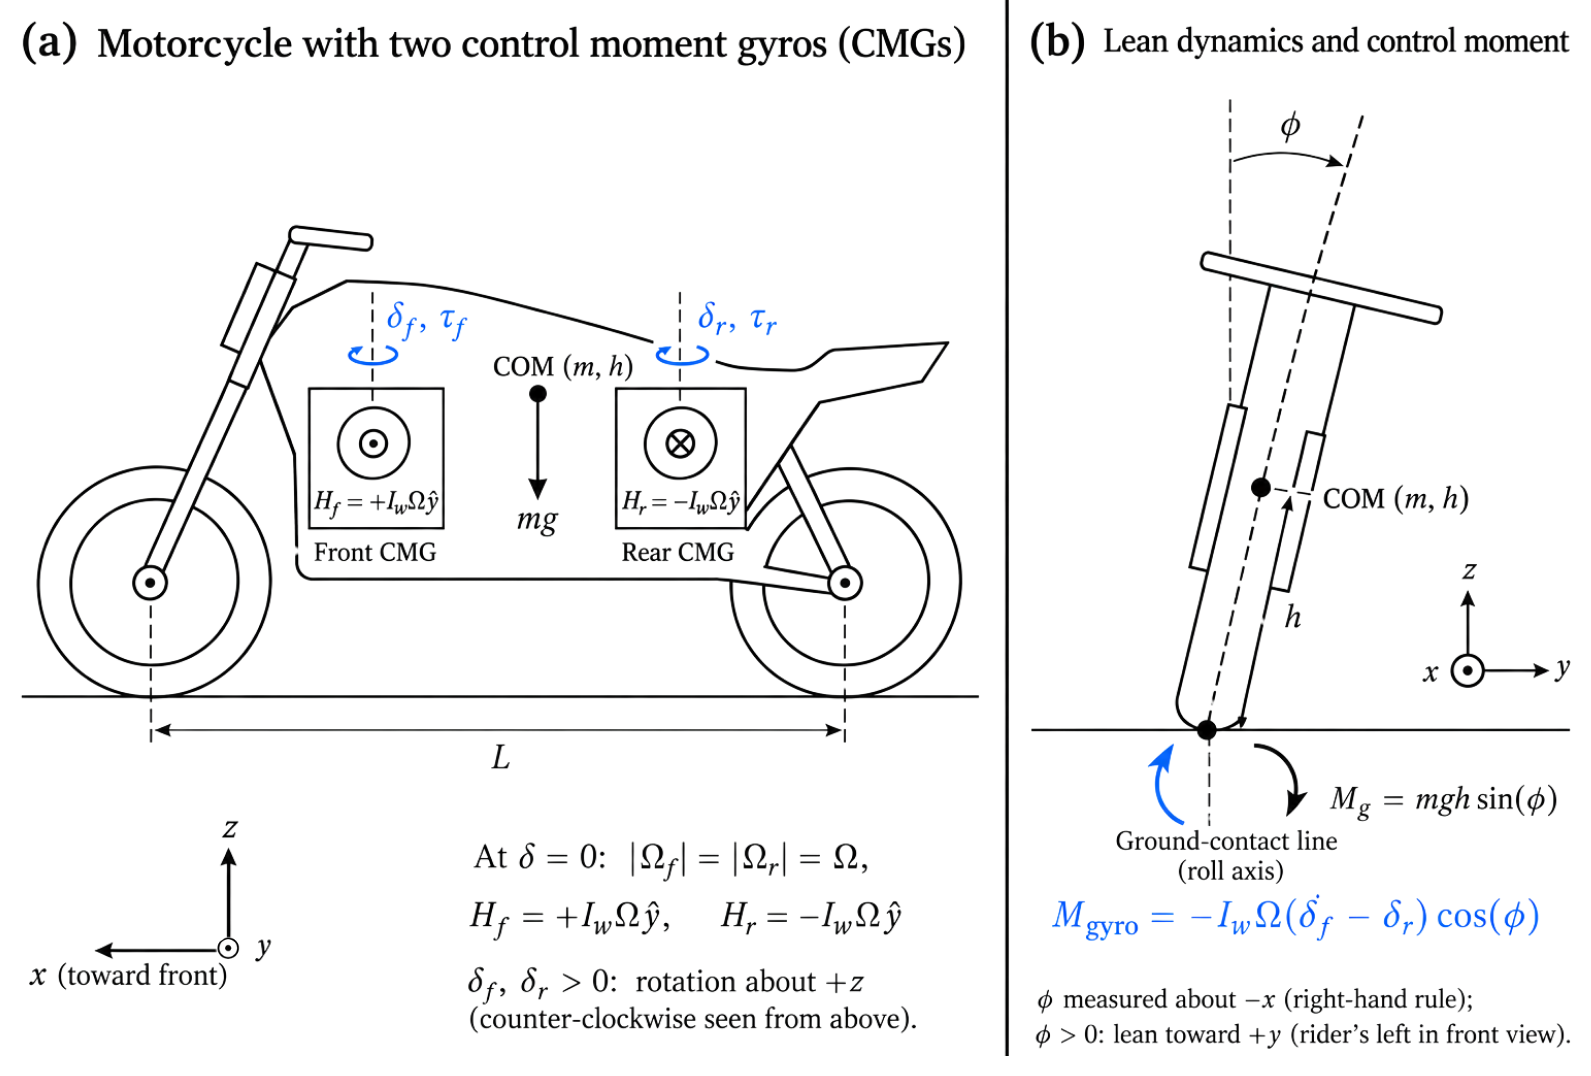
\includegraphics[width=.95\linewidth]{figs/fig1_configuration.png}
\caption{Motorcycle with two control-moment gyros. (a) Side view: front and rear CMG gimbals ($\delta_f,\tau_f$ and $\delta_r,\tau_r$), center of mass at height $h$, wheelbase $L$, counter-rotating rotor momenta. (b) Front view: gravity moment $M_g=mgh\sin\phi$ and control moment $M_{\rm gyro}=-I_w\Omega(\dot\delta_f-\dot\delta_r)\cos\phi$ of the reduced model; $\phi>0$ is a lean toward $+y$.}\label{fig:config}
\end{figure}

\begin{table}[t]\centering\small
\caption{Nominal reduced-order simulation parameters.}\label{tab:par}
\begin{tabular}{lll}\toprule
Parameter & Symbol & Nominal value\\\midrule
Total mass & $m$ & \SI{85}{kg}\\
Center-of-mass height & $h$ & \SI{0.50}{m}\\
Gravity & $g$ & \SI{9.81}{m.s^{-2}}\\
Rotor axial inertia & $I_w$ & \SI{0.50}{kg.m^2}\\
Rotor speed magnitude & $\Omega$ & \SI{200}{rad.s^{-1}}\\
Gimbal inertia & $I_\delta$ & \SI{0.10}{kg.m^2}\\
Gimbal damping rate & $c$ & \SI{2}{s^{-1}}\\
Reference wheelbase & $L$ & \SI{1.20}{m}\\
Sampling time & $T_s$ & \SI{0.01}{s}\\
Torque bound & $\tau_{\max}$ & \SI{50}{N.m}\\
Gimbal bounds & $|\delta_i|,|\dot\delta_i|$ & $\pi/2$ rad, 20 rad\,s$^{-1}$\\\bottomrule
\end{tabular}
\end{table}

\subsection{Constrained nominal MPC teacher}
Let $a=mgh/I_\phi$ and $b=I_w\Omega/I_\phi$ ($a\approx\SI{19.62}{s^{-2}}$, $b\approx\SI{4.706}{s^{-1}}$). With $\psi=\dot\delta_f-\dot\delta_r$, Eq.~\eqref{eq:roll} gives $\partial\ddot\phi/\partial\phi=a\cos\phi+b\psi\sin\phi$. At each control step the predictive model is linearized about the current (for EKF--MPC: estimated) roll angle $\phi_0$ with zero gimbal angles, rates and torque, $\bm x_0=[\phi_0,0,0,0,0,0]^\top$, $\bm u_0=\bm 0$. There $\psi_0=0$, so $(A_c)_{21}=a\cos\phi_0$ with no neglected term. The affine offset $\bm b_c=\bm f(\bm x_0,\bm 0)-A_c\bm x_0=[0,\,a(\sin\phi_0-\phi_0\cos\phi_0),0,0,0,0]^\top$ is held constant over the sampling interval, and $\dot{\bm x}\approx A_c\bm x+B_c\bm u+\bm b_c$ is discretized by zero-order hold with an augmented matrix exponential, which is exact for the affine model itself. The model is applied to the actual state, whose gimbal rates are generally non-zero; it freezes the roll dependence at $\phi_0$ and omits the curvature of the gravity term and the bilinear coupling $b\psi\sin\phi_0(\phi-\phi_0)$, so it is not an exact representation of Eqs.~\eqref{eq:roll}--\eqref{eq:gimbal}. As a diagnostic on 4{,}800 states from 200 closed-loop trajectories of a regulator built on the same model (not the evaluation rollouts), the largest 20-step open-loop roll-angle prediction error was \num{5.2e-3}\,rad (95th percentile \num{3.3e-4}\,rad); the omitted bilinear term stayed below 8.4\% of the magnitude of the gravity and gyroscopic terms (95th percentile 1.4\%), and including the full Jacobian $b\psi_0\sin\phi_0$ was not more accurate (largest error \num{1.1e-2}\,rad). The Jacobians at $\bm x_0$ are, with $a=mgh/I_\phi$ and $b=I_w\Omega/I_\phi$,
\begin{equation}
A_c(\bm x_0)=\left.\frac{\partial\bm f}{\partial\bm x}\right|_{\bm x_0}=\begin{bmatrix}
0&1&0&0&0&0\\
a\cos\phi_0&0&0&0&-b\cos\phi_0&b\cos\phi_0\\
0&0&0&0&1&0\\
0&0&0&0&0&1\\
0&0&0&0&-c&0\\
0&0&0&0&0&-c\end{bmatrix},\qquad B_c=G.\label{eq:Ac}
\end{equation}
For the zero-order-hold discretization with sampling time $T_s$, the augmented matrix exponential
\begin{equation}
\exp\!\left(\begin{bmatrix}A_c&B_c&\bm b_c\\0_{2\times6}&0_{2\times2}&0_{2\times1}\\0_{1\times6}&0_{1\times2}&0\end{bmatrix}T_s\right)=\begin{bmatrix}A_d&B_d&\bm b_d\\0&I_2&0\\0&0&1\end{bmatrix}
\end{equation}
yields the predictive model $\bm x_{j+1}=A_d\bm x_j+B_d\bm u_j+\bm b_d$ used in Eq.~\eqref{eq:mpc}.

With tracking error $\bm z_k=\bm x_k-\bm x_k^{\rm ref}$, the teacher solves
\begin{equation}
\min_{\{\bm u_j\}}\sum_{j=0}^{N-1}\Big(\bm z_j^\top Q\bm z_j+\bm u_j^\top R\bm u_j+\tfrac12\|\bm u_j-\bm u_{j-1}\|_2^2\Big)+\bm z_N^\top P\bm z_N,\label{eq:mpc}
\end{equation}
subject to the affine dynamics, $\|\bm u_j\|_\infty\le\SI{50}{N.m}$, $|\delta_i|\le\pi/2$ and $|\dot\delta_i|\le\SI{20}{rad.s^{-1}}$, with nominal horizon $N=20$,
\begin{equation}
Q=\mathrm{diag}(70.7107,\,7.0711,\,22.3607,\,22.3607,\,2.2361,\,2.2361),\qquad R=0.31623\,I_2,
\end{equation}
and a terminal cost $P$ from a Riccati equation. The convex quadratic program is solved with CVXPY/OSQP with warm starting \cite{stellato2020osqp}. These are design weights (geometric means of the weight ranges of the original design environment), not identified physical parameters.

%==============================================================
\section{Controller architectures}
\subsection{Neural MPC, Pure SAC and residual SAC}\label{sec:nn}
\paragraph{Design rationale.}
Online constrained MPC handles actuator and gimbal limits but requires a quadratic program at every step. To combine its deterministic constraint handling with the execution speed of neural networks, we adopt a two-tier architecture: an offline-distilled neural MPC provides the fast nominal action, and a bounded residual SAC policy is examined as a compensator for plant mismatch and measurement degradation (Q2). Preliminary experiments in which SAC selected the MPC weights and horizon online gave no tracking benefit over fixed weights and were not pursued.

Pure SAC denotes a SAC policy mapping observations directly to torque (normalized action scaled to $\pm\SI{50}{N.m}$). The neural MPC imitates the first torque of the MPC teacher. Two networks are used and always identified explicitly:
\begin{itemize}
\item the \emph{10-input network}, $\bm o=[\phi,\dot\phi,\delta_f,\delta_r,\dot\delta_f,\dot\delta_r,v,\alpha,\phi_d,e_\phi]^\top$ (six states, speed, a steering-related quantity, desired roll, roll error), a 10--256--256--128--2 perceptron with output $\bm u_{NN}=50\tanh(\cdot)$; it is used in Tables~\ref{tab:val10}, \ref{tab:cl}, the fixed-horizon residual family and the 34-scenario benchmark;
\item the \emph{13-input (horizon-conditioned) network}, which additionally receives the previous torque $\bm u_{k-1}$ and the selected horizon $N$ (Fig.~\ref{fig:arch}); it is the base of the adaptive-horizon residual family and, with $N=20$ fixed, the ``Neural MPC'' of Tables~\ref{tab:focus}, \ref{tab:abl} and \ref{tab:abl2}.
\end{itemize}
During neural inference the MPC quadratic program is not solved.

\paragraph{Distillation of the 10-input network.}
Teacher rollouts were generated under healthy nominal dynamics from three initial-condition buckets (nominal, moderately perturbed, hard conditions near the stability boundary; probabilities $0.4/0.3/0.3$), one sample per plant step. Only solver statuses \emph{optimal} and \emph{optimal inaccurate} were retained; failed solves (executed by the teacher as zero torque) were excluded so that the network does not learn zero torque where the solver failed. The training set comprises 1{,}500 episodes (747{,}522 attempted transitions, 729{,}978 retained) and the independent validation set 200 episodes with distinct seeds (99{,}009 attempted, 97{,}454 retained); teacher labels never exceeded about \SI{21.2}{N.m}. The loss is a squared error normalized by the label standard deviation $\sigma_u=\SI{0.723}{N.m}$ and weighted by three for $|\phi|>15^\circ$,
\begin{equation}
\mathcal L(\theta)=\frac1B\sum_{i=1}^B w_i\,\frac12\sum_{j\in\{f,r\}}\Big(\frac{u^{NN}_{ij}-u^{MPC}_{ij}}{\sigma_u}\Big)^2,\quad w_i=\begin{cases}3,&|\phi_i|>15^\circ\\1,&\text{otherwise,}\end{cases}\label{eq:loss}
\end{equation}
minimized with Adam (learning rate $10^{-3}$, cosine-annealed to 1\% over at most 100 epochs, batch 1{,}024, gradient-norm clipping at 5, early-stopping patience 15), selecting the checkpoint with the lowest validation RMSE (\SI{0.0375}{N.m}); patience was not triggered. Table~\ref{tab:val10} gives the held-out errors. The policy preserves front/rear torque symmetry (mean $|\tau_f+\tau_r|=\SI{8e-8}{N.m}$).

\begin{table}[t]\centering\small
\caption{Held-out validation torque error of the distilled 10-input neural MPC (N\,m).}\label{tab:val10}
\begin{tabular}{lrcccc}\toprule
Subset & $n$ & RMSE & MAE & P95 $|e|$ & P99 $|e|$\\\midrule
All & 97{,}454 & 0.0375 & 0.0253 & 0.080 & 0.124\\
$|\phi|\le15^\circ$ & 91{,}186 & 0.0368 & 0.0247 & 0.079 & 0.122\\
$|\phi|>15^\circ$ & 6{,}268 & 0.0465 & 0.0339 & 0.097 & 0.146\\
$|\phi|>25^\circ$ & 1{,}784 & 0.0499 & 0.0350 & 0.106 & 0.164\\\bottomrule
\end{tabular}
\end{table}

Offline error alone cannot establish closed-loop stability, so the network was compared with the teacher on the same seeds, initial conditions, reference, plant and noise (Table~\ref{tab:cl}; 100 seeds per condition, healthy plant). Episode completion was identical (99/100 nominal, 100/100 hard; the single nominal failure is shared and occurs after seven steps), roll-tracking RMSE agreed within \SI{0.0003}{rad}, neither controller saturated, and the mean paired roll-trajectory disagreement was $0.055^\circ$ (nominal) and $0.075^\circ$ (hard), worst episode $0.55^\circ$. Mean command-computation time fell from \SI{17.3}{ms} and \SI{16.9}{ms} to \SI{0.095}{ms} and \SI{0.093}{ms}, a factor of 181.0 and 181.9. The teacher's solver returned a failed status in 1.2\% (nominal) and 2.6\% (hard) of the steps, whereas the network has no such failures; the teacher's mean time includes those calls. The speed-up is specific to the tested CPU implementation (PyTorch inference against CVXPY/OSQP) and the command-computation path; it is neither hardware-independent nor a worst-case real-time guarantee. The acceptance gate (completion drop $\le0.03$, survivor RMSE and mean peak-roll ratios $\le1.25$) is an empirical criterion, not a formal equivalence test, and was applied only to the healthy plant.

\begin{table}[t]\centering\small
\caption{Paired healthy-plant closed-loop comparison of the teacher MPC and the distilled 10-input neural MPC (100 seeds per condition). Time is the mean command-computation time; Median/P95/Max are episode-level statistics (median of 100 episode means, mean of per-episode 95th percentiles, maximum over all steps).}\label{tab:cl}
\resizebox{\linewidth}{!}{%
\begin{tabular}{llcccccccc}\toprule
Cond. & Controller & Surv. & RMSE (rad) & Peak $|\phi|$ ($^\circ$) & $\|u\|$ & Mean (ms) & Median (ms) & P95 (ms) & Max (ms)\\\midrule
Nominal & MPC & 0.99 & 0.1976 & 22.38 & 0.4433 & 17.262 & 17.80 & 27.40 & 135.77\\
Nominal & Neural MPC & 0.99 & 0.1974 & 22.35 & 0.4374 & 0.095 & 0.088 & 0.138 & 1.39\\
Hard & MPC & 1.00 & 0.1918 & 21.95 & 0.2957 & 16.885 & 14.85 & 29.77 & 68.50\\
Hard & Neural MPC & 1.00 & 0.1915 & 21.91 & 0.2914 & 0.093 & 0.090 & 0.137 & 1.04\\\bottomrule
\end{tabular}}
\end{table}

\paragraph{Distillation of the 13-input network.}
Teacher rollouts used the same MPC at $N\in\{10,20,30,40\}$. For each of 375 base seeds all four horizons were rolled out from the same initial condition (1{,}500 teacher episodes, 747{,}634 attempted transitions); initial-condition buckets were cycled in equal proportions and the horizon enters as the raw value $N$. Only samples with status \emph{optimal} were retained (747{,}537 remain; 97 excluded, 0.013\%). The loss is Eq.~\eqref{eq:loss}; training used AdamW (learning rate $10^{-3}$, weight decay $10^{-5}$), batch 1{,}024, reduce-on-plateau scheduling (factor 0.5, patience 7), gradient clipping at 5, at most 150 epochs and early-stopping patience 20, with normalization statistics from the training set only. The best validation checkpoint was reached near the epoch cap, so training was limited by the epoch budget. The validation set comes from 50 independent base seeds (200 teacher episodes, none ended in a crash; 99{,}990 of 100{,}000 samples retained). Its RMSE is \SI{0.0293}{N.m} (Table~\ref{tab:val13}). Unlike the 10-input network, torque symmetry is only approximate (mean $|\tau_f+\tau_r|=\SI{0.0116}{N.m}$).

\begin{table}[t]\centering\small
\caption{Held-out validation torque error of the 13-input neural MPC (N\,m).}\label{tab:val13}
\begin{tabular}{lrcccc}\toprule
Subset & $n$ & RMSE & MAE & P95 $|e|$ & P99 $|e|$\\\midrule
All & 99{,}990 & 0.0293 & 0.0162 & 0.054 & 0.111\\
$N=10$ & 24{,}992 & 0.0452 & 0.0259 & 0.086 & 0.159\\
$N=20$ & 24{,}998 & 0.0274 & 0.0178 & 0.050 & 0.095\\
$N=30$ & 25{,}000 & 0.0192 & 0.0116 & 0.035 & 0.073\\
$N=40$ & 25{,}000 & 0.0161 & 0.0093 & 0.027 & 0.061\\
$|\phi|\le15^\circ$ & 96{,}860 & 0.0260 & 0.0151 & 0.049 & 0.100\\
$|\phi|>15^\circ$ & 3{,}130 & 0.0803 & 0.0476 & 0.143 & 0.249\\
$|\phi|>25^\circ$ & 732 & 0.1118 & 0.0633 & 0.172 & 0.269\\\bottomrule
\end{tabular}
\end{table}

\paragraph{Residual design.}
The residual architecture (Fig.~\ref{fig:arch}) retains the neural baseline and adds a bounded learned correction,
\begin{equation}
\bm u_k=\mathrm{clip}\big(\bm u_{NN}(\bm o_k)+\lambda\,\bm a_{\rm SAC}(\bm o_k^{\rm res}),\,-\tmax,\,\tmax\big).\label{eq:res}
\end{equation}
The correction is a squashed policy output with an explicit bound. Writing $\bm s_k$ for the residual observation $\bm o_k^{\rm res}$,
\begin{equation}
\Delta\bm u_k=\tau^{\rm res}_{\max}\,\bm a_k,\quad \bm a_k=\tanh\!\big(\bm\mu_\theta(\bm s_k)\big)\ \text{(or }\tanh(\bm\mu_\theta+\bm\sigma_\theta\odot\bm\xi)\text{ when sampled)},\qquad \tau^{\rm res}_{\max}=\lambda,\label{eq:dures}
\end{equation}
so that, whether the action is sampled or deterministic,
\begin{equation}
\|\Delta\bm u_k\|_\infty\le\tau^{\rm res}_{\max}=\SI{5}{N.m}=0.1\,\tau_{\max}.\label{eq:resbound}
\end{equation}
With $\pi_{\rm distill}(\bm x_k)=\bm u_{NN}(\bm o_k)$, Eq.~\eqref{eq:res} is the clipped sum $\bm u_k=\mathrm{clip}(\pi_{\rm distill}+\Delta\bm u_k)$. Because componentwise clipping is $1$-Lipschitz, the applied torque differs from the clipped baseline torque by at most the residual bound,
\begin{equation}
\|\bm u_k-\mathrm{clip}(\pi_{\rm distill}(\bm x_k),-\tmax,\tmax)\|_\infty\le\tau^{\rm res}_{\max},
\end{equation}
so the learned policy can neither exceed the physical torque limit nor move the command further from the baseline than $\tau^{\rm res}_{\max}$ per channel.

Two residual families appear and must not be conflated.
\begin{enumerate}
\item[(i)] \emph{Fixed-horizon residual (34-scenario benchmark):} base is the 10-input network; SAC observation $\bm o_k^{\rm res}=[\bm z_k^\top,(\bm u_{NN,k}/U_{\rm ref})^\top]^\top$ (12 components, $U_{\rm ref}=\SI{5}{N.m}$); action $\bm a_k\in[-1,1]^2$ scaled by $\lambda=\SI{5}{N.m}$, i.e.\ a per-channel authority of 10\% of $\tmax$.
\item[(ii)] \emph{Adaptive-horizon residual (focused holdout and cross-simulator study):} base is the 13-input network; the 15-dimensional observation holds the ten components $\bm z_k$, the previous applied torque and the current base output (both divided by $U_{\rm ref}$), and the horizon index scaled to $[-1,1]$. The action $\bm a_t=[a_f,a_r,a_h]$ is three-dimensional with $\lambda=\SI{5}{N.m}$; the horizon channel selects $N\in\{10,20,30,40\}$ through $k=\min(\lfloor\tfrac12(a_h+1)\cdot4\rfloor,3)$. In a 10-episode check the mean selected horizon was 28.2--29.0 with about 300 switches per episode, so the channel is actively used (this does not show adaptation is beneficial).
\end{enumerate}
Because the adaptive residual may still select the horizon at $\lambda=0$, it is not by itself equivalent to the standalone neural MPC; Section~\ref{sec:lambda} separates both contributions.

\begin{figure}[t]\centering
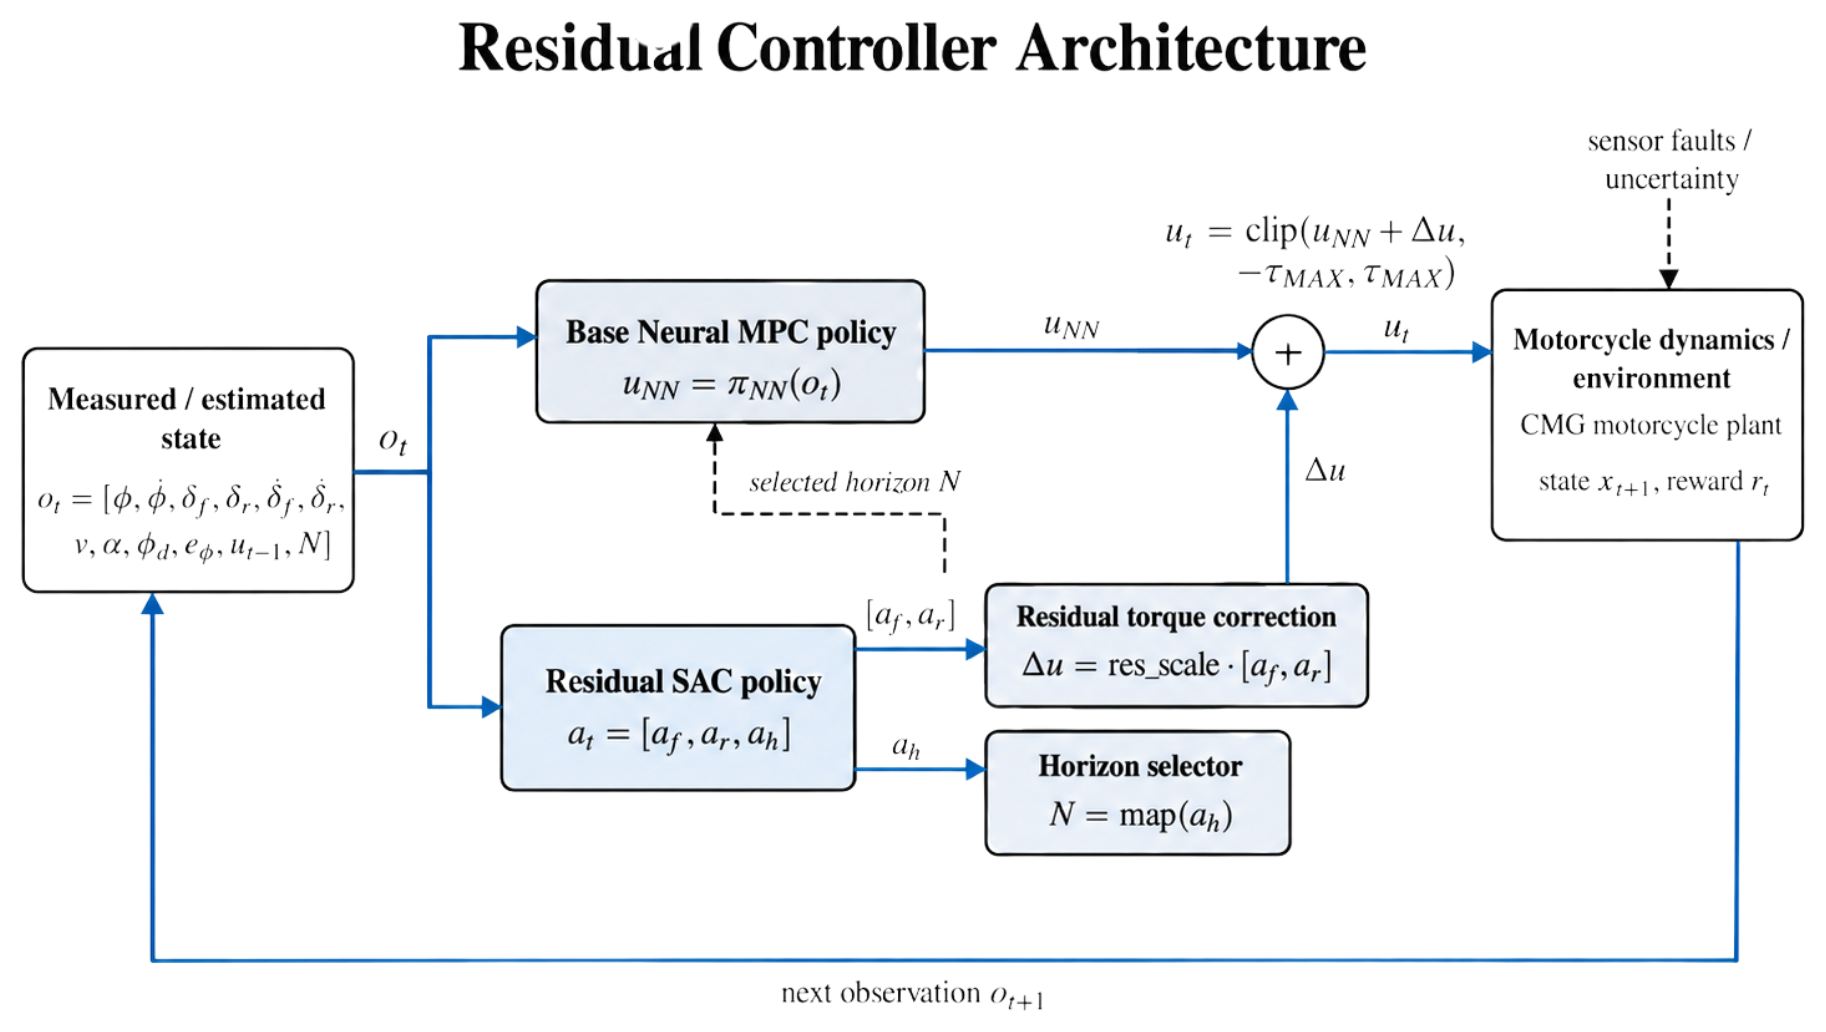
\includegraphics[width=.95\linewidth]{figs/fig2_architecture.png}
\caption{Residual controller architecture. The measured/estimated observation $\bm o_t$ feeds the base neural MPC ($\bm u_{NN}=\pi_{NN}(\bm o_t)$) and the residual SAC policy ($\bm a_t=[a_f,a_r,a_h]$). The torque channels give $\Delta\bm u=\text{res\_scale}\cdot[a_f,a_r]$, the horizon channel selects $N=\mathrm{map}(a_h)$, and the applied torque is $\bm u_t=\mathrm{clip}(\bm u_{NN}+\Delta\bm u,-\tmax,\tmax)$. Sensor faults and uncertainty enter the plant loop. The base network has 13 inputs; the adaptive residual observation has 15 components.}\label{fig:arch}
\end{figure}

\paragraph{Training of the adaptive-horizon residual policies.}
Five policies (training seeds 101, 202, 303, 404, 505) use SAC (learning rate $3\times10^{-4}$, batch 256, replay buffer $5\times10^5$, 2{,}000 warm-up steps, $\gamma=0.99$, $\tau=0.005$, two hidden layers of 256 units) with running normalization of observations and rewards (clip 10) and a residual-initialized actor (output weights scaled by 0.01, zero bias, horizon bias at the $N=20$ bin). Each episode samples the rotor-inertia scale uniformly from $\{1.0,0.8,0.7,0.6,0.5\}$ and the bucket with probabilities $0.4/0.3/0.3$, with the neural MPC frozen; the training range therefore ends at 0.5. \emph{No measurement fault is injected during training}, so all fault scenarios are zero-shot for these policies. Checkpoints were scored by $\overline{\rm surv}-0.5\,\overline{\rm RMSE}$ on 30 fixed episodes per scale every 10{,}000 steps. Seeds 101, 202 and 303 were trained for 300{,}000 steps and continued to 1{,}000{,}000 steps with the replay buffer reloaded (their ``best'' checkpoint is the best of the continuation); seeds 404 and 505 were trained from scratch to 1{,}000{,}000 steps. The training budget is therefore not identical across seeds (Table~\ref{tab:steps}). The Pure SAC policies of the focused holdout (seeds 11, 22, 33, 44, 55) were trained for 1{,}000{,}000 steps. The checkpoints of seeds 404 and 505 were trained under NumPy~2 and converted for evaluation under NumPy~1.26 (Section~\ref{sec:limits}). On an independent check of 510 episodes (34 scenarios), the best and final checkpoints of seed 404 reached 75.9\% and 74.7\% survival, and the best checkpoint of seed 505 74.5\%.

\begin{table}[t]\centering\small
\caption{Training steps of the best-score and final SAC checkpoints. The fixed-horizon residual of Tables~\ref{tab:34} and \ref{tab:iw} has its best checkpoint at 875{,}000 and its final at 1{,}000{,}000 steps.}\label{tab:steps}
\begin{tabular}{crrcrr}\toprule
Residual seed & best & final & Pure SAC seed & best & final\\\midrule
101 & 600{,}000 & 1{,}000{,}000 & 11 & 710{,}000 & 1{,}000{,}000\\
202 & 730{,}000 & 1{,}000{,}000 & 22 & 620{,}000 & 1{,}000{,}000\\
303 & 980{,}000 & 1{,}000{,}000 & 33 & 980{,}000 & 1{,}000{,}000\\
404 & 590{,}000 & 1{,}000{,}000 & 44 & 840{,}000 & 1{,}000{,}000\\
505 & 890{,}000 & 1{,}000{,}000 & 55 & 930{,}000 & 1{,}000{,}000\\\bottomrule
\end{tabular}
\end{table}

\paragraph{Reward and the fixed-horizon family.}
The fixed-horizon family was trained with the clipped reward
\begin{equation}
\begin{split}
r_k&=\mathrm{clip}\Big(1+e^{-20e_{\phi,k}^2}-0.05|\dot\phi_k|-w_u\Big\|\tfrac{\bm u_k}{\tmax}\Big\|^2\\
&\qquad-w_{\Delta u}\Big\|\tfrac{\bm u_k-\bm u_{k-1}}{2\tmax}\Big\|^2-w_a\|\bm a_k\|^2,\,0,\,2\Big),\quad r_k^{\rm crash}=-C_{\rm crash}.
\end{split}\label{eq:rew}
\end{equation}
In all reported runs the penalty weights and the crash reward take the values of Table~\ref{tab:rew}, so Eq.~\eqref{eq:rew} reduces to $\mathrm{clip}(1+e^{-20e_\phi^2}-0.05|\dot\phi|,0,2)$ with a crash reward of $-1000$. For the adaptive-horizon family the expression is the same, with the residual penalty $w_a$ applied to the two torque channels only and no term involving the horizon channel.

\begin{table}[t]\centering\small
\caption{Reward parameters of Eq.~\eqref{eq:rew} in all reported runs.}\label{tab:rew}
\begin{tabular}{lc}\toprule
Parameter & Value\\\midrule
Control-effort weight $w_u$ & 0\\
Control-rate weight $w_{\Delta u}$ & 0\\
Action-magnitude weight $w_a$ & 0\\
Crash reward $C_{\rm crash}$ & 1000\\\bottomrule
\end{tabular}
\end{table}

The fixed-horizon residual used in Tables~\ref{tab:34}, \ref{tab:iw} and \ref{tab:app} is the best-score checkpoint (875{,}000 of 1{,}000{,}000 steps) of one run with $\lambda=\SI{5}{N.m}$, trained with the rotor-inertia scale drawn uniformly from $\{1.0,0.5,0.45,0.42,0.4\}$ and bucket probabilities $0.4/0.3/0.3$ with the neural MPC frozen; checkpoints were scored every 25{,}000 steps on 20 fixed episodes per scale. The scale list was chosen after pilot sweeps of the neural MPC at reduced inertia (Section~\ref{sec:inertia}), i.e.\ it targets the range in which the neural MPC fails. Because the observation layouts and action scalings of the two families differ, the two cohorts are reported separately. Checkpoint-specific observation normalization is a prerequisite for reproducing inference results.

\subsection{Robust EKF and online MPC}\label{sec:ekf}
Let the discrete dynamics and the six-channel sensor satisfy
\begin{equation}
\bm x_{k+1}=\bm f_d(\bm x_k,\bm u_k)+\bm w_k,\qquad \bm y_k=\bm h(\bm x_k)+\bm v_k+\bm f_k,\label{eq:meas}
\end{equation}
where $\bm h(\bm x)=\bm x$ (so $H_k=I_6$), $\bm w_k\sim\mathcal N(\bm 0,Q_{\rm EKF})$, $\bm v_k\sim\mathcal N(\bm 0,R_{\rm EKF})$ is the filter's noise model, and $\bm f_k$ is the sensor-fault vector (dropout, hold, stuck value; Section~\ref{sec:protocol}) acting on the roll angle and roll rate channels only. The prediction uses the nominal model and the discrete Jacobian $F_k$ of the MPC linearization:
\begin{equation}
\hat{\bm x}_{k|k-1}=\bm f_d(\hat{\bm x}_{k-1|k-1},\bm u_{k-1}),\qquad P_{k|k-1}=F_kP_{k-1|k-1}F_k^\top+Q_{\rm EKF}.
\end{equation}
With innovation $\tilde{\bm y}_k=\bm y_k-\bm h(\hat{\bm x}_{k|k-1})$ and innovation covariance $S_k=H_kP_{k|k-1}H_k^\top+R_{\rm EKF}$, let $\tilde{\bm y}_k^{r}$ and $S_k^{r}$ denote the roll-angle/roll-rate sub-vector ($2\times1$) and its $2\times2$ block. The roll channels are validated by the squared Mahalanobis distance
\begin{equation}
d_k^2=(\tilde{\bm y}_k^{r})^\top (S_k^{r})^{-1}\tilde{\bm y}_k^{r},\label{eq:maha}
\end{equation}
which is $\chi^2_2$-distributed under the nominal (fault-free, Gaussian) hypothesis, and is compared with $\gamma=\chi^2_{2,\,0.01}=9.21$ (99\% confidence level). A stale-data indicator $\varsigma_k\in\{0,1\}$ equals one if the delivered roll angle and rate have changed by no more than $\epsilon_s=10^{-10}$ with a zero reported roll rate for $N_s=2$ consecutive samples. The roll channels are rejected at step $k$ when $r_k=\mathbb 1[d_k^2>\gamma\ \lor\ \varsigma_k=1]$. The set of accepted channels is $\mathcal A_k=\{3,4,5,6\}\cup\{1,2\ \text{if}\ r_k=0\}$: \emph{the gimbal channels are always used}, so on rejection the update is a gimbal-only correction rather than a pure prediction. With $H_{\mathcal A}$, $R_{\mathcal A}$ the rows/blocks selected by $\mathcal A_k$,
\begin{align}
K_k&=P_{k|k-1}H_{\mathcal A}^\top\big(H_{\mathcal A}P_{k|k-1}H_{\mathcal A}^\top+R_{\mathcal A}\big)^{-1},\qquad
\hat{\bm x}_{k|k}=\hat{\bm x}_{k|k-1}+K_k\tilde{\bm y}_{k,\mathcal A},\label{eq:upd}\\
P_{k|k}&=(I-K_kH_{\mathcal A})P_{k|k-1}(I-K_kH_{\mathcal A})^\top+K_kR_{\mathcal A}K_k^\top\quad\text{(Joseph form).}\label{eq:joseph}
\end{align}
For the roll block alone this is the conditional rule $\hat{\bm x}_{k|k}=\hat{\bm x}_{k|k-1}+K_k\tilde{\bm y}_k$ if $d_k^2\le\gamma$ and no roll correction otherwise.

\paragraph{Covariance recovery.} Let $n_k=(n_{k-1}+1)\,r_k$ count consecutive roll rejections. To keep the filter receptive when the roll sensor returns after a long outage, the roll rows and columns of the covariance are inflated after every $N_{\rm th}=5$-th consecutive rejection and the roll variances are capped:
\begin{equation}
P_{k|k}\leftarrow D_k P_{k|k}D_k,\quad D_k=\mathrm{diag}\big(\sqrt{\alpha_k},\sqrt{\alpha_k},1,1,1,1\big),\quad
\alpha_k=\begin{cases}\kappa,& n_k>0\ \text{and}\ n_k\bmod N_{\rm th}=0,\\1,&\text{otherwise,}\end{cases}\label{eq:infl}
\end{equation}
followed by $[P_{k|k}]_{ii}\leftarrow\min\{[P_{k|k}]_{ii},\bar p\}$ for $i\in\{1,2\}$, with $\kappa=4$ and $\bar p=1.0$. Thus the roll--roll covariance block grows by the factor $\kappa$ (roll--other cross-covariances by $\sqrt\kappa$), and the roll variances remain bounded. Algorithm~\ref{alg:ekfmpc} summarizes one control step.

\begin{algorithm}[t]
\caption{One step of EKF--MPC with robust roll-channel validation}\label{alg:ekfmpc}
\begin{algorithmic}[1]
\Require $\hat{\bm x}_{k-1|k-1},P_{k-1|k-1},\bm u_{k-1},\bm y_k,n_{k-1}$
\State Predict: $\hat{\bm x}_{k|k-1},P_{k|k-1}$
\State $\tilde{\bm y}_k\gets\bm y_k-\hat{\bm x}_{k|k-1}$; compute $d_k^2$ (Eq.~\eqref{eq:maha}) and $\varsigma_k$
\State $r_k\gets\mathbb 1[d_k^2>\gamma\lor\varsigma_k=1]$; $n_k\gets(n_{k-1}+1)r_k$
\State Update with accepted set $\mathcal A_k$ (Eqs.~\eqref{eq:upd}--\eqref{eq:joseph})
\If{$n_k>0$ \textbf{and} $n_k\bmod N_{\rm th}=0$} inflate and cap roll covariance (Eq.~\eqref{eq:infl})\EndIf
\State Linearize at $\phi_0=\hat\phi_{k|k}$, discretize (Section 3.2), solve the QP for $\bm u_{0:N-1}$
\State Apply $\bm u_k\gets\bm u_0$ (zero torque if the solver fails)
\end{algorithmic}
\end{algorithm}

The filter is initialized from the first six-channel sensor sample, which may itself be corrupted; the true state is used only for metrics. The noise settings are standard deviations from which $Q_{\rm EKF}=\mathrm{diag}(\sigma_Q^2)$, $R_{\rm EKF}=\mathrm{diag}(\sigma_R^2)$ and $P_0=\mathrm{diag}(\sigma_P^2)$ are formed:
\begin{align}
\sigma_Q&=(0.002,\,0.05,\,0.005,\,0.005,\,0.1,\,0.1),\\
\sigma_R&=(0.01,\,0.1,\,0.005,\,0.005,\,0.05,\,0.05),\\
\sigma_P&=(0.05,\,0.5,\,0.05,\,0.05,\,0.5,\,0.5).
\end{align}
The robustness parameters are $\gamma=9.21$, $\epsilon_s=10^{-10}$, $N_s=2$, $N_{\rm th}=5$, $\kappa=4$ and $\bar p=1.0$ (Eqs.~\eqref{eq:maha}--\eqref{eq:infl}). These settings were selected in a pilot on seeds 77000--77004 and then frozen; the evaluation seeds 78000--78099 do not overlap. The online MPC quadratic program is solved with OSQP ($\epsilon_{\rm abs}=\epsilon_{\rm rel}=10^{-4}$, at most 4{,}000 iterations, warm starting); a failed solve is executed as zero torque. The hard gimbal-rate constraint of the teacher and OSQP's automatic step-size selection are retained. State estimates, not the corrupted roll observations, are passed to the online MPC, evaluated at $N=10,20,30,40$.

A smoke test (seed 78000, $N=20$, five scenarios) served as a structural integrity check only and no parameter was changed afterwards. All 6{,}000 horizon--scenario episodes of Section~\ref{sec:results} come from one complete run of this frozen configuration (1{,}500 verified unique episode keys per horizon); a complete repeat is described in Section~\ref{sec:horizon}. A paired fresh-run check ($N=20$, seeds 77000--77004, 45 episodes) found that the baseline mode of the evaluation module (stale-data detection and covariance recovery off) returned values identical to the original estimator script for all ten compared metrics (tolerance $10^{-6}$). The reported runs use the combined mode, which adds both safeguards.

\subsection{Boundedness analysis}\label{sec:bound}
A Lyapunov certificate for the learned components is not available. What can be stated rigorously is a \emph{conditional} result, in which the stability property of the baseline is an explicit assumption, together with structural bounds that the architecture does enforce.

\begin{lemma}[Gated update]\label{lem:gate}
Consider the update of Eqs.~\eqref{eq:maha}--\eqref{eq:infl} with $R_{\rm EKF}\succ0$ and $P_{k|k-1}\succeq0$.
\begin{enumerate}
\item[(i)] \emph{Bounded accepted innovation.} If the roll channels are accepted ($r_k=0$), then $\|\tilde{\bm y}^r_k\|_2^2\le\gamma\,\lambda_{\max}(S^r_k)$ with $\gamma=9.21$; no accepted roll sample can lie farther from the prediction than $\sqrt{\gamma\lambda_{\max}(S_k^r)}$.
\item[(ii)] \emph{Covariance consistency.} $P_{k|k}\succeq0$ for any gain $K_k$, including after the inflation of Eq.~\eqref{eq:infl}.
\item[(iii)] \emph{Open-loop growth during rejection.} The roll states are not observable from the gimbal channels, since the gimbal dynamics do not depend on $\phi$ or $\dot\phi$. During $n$ consecutive roll rejections the roll covariance block is therefore driven by prediction alone, $P^r_{+}=\Phi P^r\Phi^\top+Q^r_{\rm EKF}$ (up to coupling through the measured gimbal rates), with $\Phi\approx\exp(A^rT_s)$, $A^r=\begin{bmatrix}0&1\\a\cos\phi_0&0\end{bmatrix}$ whose eigenvalues are $\pm\sqrt{a\cos\phi_0}$. At $\phi_0=0$ the covariance can grow by up to $e^{2\sqrt aT_s}\approx1.09$ per step, i.e.\ without bound as $n\to\infty$; the cap $\bar p$ of Eq.~\eqref{eq:infl} is what keeps the roll variances bounded.
\end{enumerate}
\end{lemma}
\begin{proof}
(i) For a symmetric positive definite $S$, $\bm v^\top S^{-1}\bm v\ge\|\bm v\|_2^2/\lambda_{\max}(S)$; combine with $d_k^2\le\gamma$. (ii) The Joseph form $(I-KH)P(I-KH)^\top+KRK^\top$ is a sum of two positive semidefinite terms for any $K$, and $D P D^\top\succeq0$ for any $D$. (iii) Linearizing the roll rows of $F_k$ about $\bm x_0$ with Eq.~\eqref{eq:Ac} gives $A^r$ and the stated eigenvalues $\pm\sqrt{a\cos\phi_0}$; the covariance recursion follows from the prediction equation when no roll measurement is applied, and $e^{2\sqrt aT_s}=e^{0.0886}\approx1.09$ for $a=19.62\,\mathrm{s^{-2}}$, $T_s=0.01$\,s.
\end{proof}

Part (iii) explains why the stale-data and recovery logic matters: with the gate alone, a long outage leaves the filter either rejecting valid data (an over-confident roll estimate) or, after unbounded variance growth, trusting corrupted samples. Lemma~\ref{lem:gate} bounds the effect of one gated sample, not of a sequence of corrupted samples that each remain inside the gate.

\begin{assumption}[ISS of the baseline loop]\label{as:iss}
Let $\bm e_k=\hat{\bm x}_{k|k}-\bm x_k$ be the estimation error and $\bm d_k=\bm u_k-\mathrm{clip}(\pi_{\rm distill}(\hat{\bm x}_k))$ the deviation of the applied torque from the baseline command. There exist a set $\Omega\subset\mathbb R^6$, a function $\beta\in\mathcal{KL}$ and $\gamma_e,\gamma_d\in\mathcal K$ such that the closed loop with the baseline controller satisfies, for all $\bm x_0\in\Omega$ and all perturbation sequences keeping the trajectory in $\Omega$,
\[
\|\bm x_k\|\le\beta(\|\bm x_0\|,k)+\gamma_e\big(\sup_{j\le k}\|\bm e_j\|\big)+\gamma_d\big(\sup_{j\le k}\|\bm d_j\|\big).
\]
\end{assumption}

\begin{proposition}[Ultimate boundedness]\label{prop:ub}
Under Assumption~\ref{as:iss}, if $\|\bm e_k\|\le\bar e$ for all $k$, then by Eq.~\eqref{eq:resbound} $\|\bm d_k\|_2\le\sqrt2\,\tau^{\rm res}_{\max}$, and the state is ultimately bounded:
\[
\limsup_{k\to\infty}\|\bm x_k\|\le\gamma_e(\bar e)+\gamma_d\big(\sqrt2\,\tau^{\rm res}_{\max}\big).
\]
\end{proposition}
\begin{proof}
$\beta(\|\bm x_0\|,k)\to0$ as $k\to\infty$, and the two suprema are bounded by $\bar e$ and $\sqrt2\tau^{\rm res}_{\max}$, respectively; take $\limsup$ in the inequality of Assumption~\ref{as:iss}.
\end{proof}

The proposition is deliberately modest: all the stabilizing content sits in Assumption~\ref{as:iss}, and the bounded residual enters only through $\gamma_d(\sqrt2\tau^{\rm res}_{\max})$. The estimator contributes Lemma~\ref{lem:gate}: a single accepted roll sample is bounded, which does not bound slowly drifting faults that stay inside the gate. One further structural fact concerns the gimbal limit. In kinematics where the roll torque of each gimbal scales with $\cos\delta_i$ (the higher-fidelity model HF-A, not Eq.~\eqref{eq:roll}), a limit $|\delta_i|\le\delta_{\max}<\pi/2$ guarantees an authority coefficient of at least $\cos\delta_{\max}$ (e.g.\ $\cos0.8=0.70$ for Stop~B); the closed limit $\pi/2$ of the reduced model gives no such lower bound, and the reduced model itself has no angle dependence at all.

\begin{remark}[Scope of the guarantee]
Assumption~\ref{as:iss} is \emph{not} verified for the learned baseline, and the paper's own results show where it fails: the neural MPC survives 0\% under burst-20 corruption on raw measurements and 0\% at 30\% of nominal rotor inertia (Table~\ref{tab:iw}); the gate alone is insufficient (Table~\ref{tab:abl}); and learned policies park the gimbals at $\pm\pi/2$ (Section~\ref{sec:mech}), where the HF-A authority vanishes. The conclusions of this paper are therefore empirical and limited to five-second episodes; Proposition~\ref{prop:ub} only clarifies which property a future certificate would have to establish.
\end{remark}

%==============================================================
\section{Fault injection and evaluation design}\label{sec:protocol}
The focused holdout uses evaluation seeds 78000--78099 across three prescribed initial-condition groups (buckets 0--2), so each of five scenarios provides 300 cases per controller instance: healthy roll measurement, roll-angle/rate dropout with probability 0.3, dropout with probability 0.5, intermittent bursts of 20 steps, and a roll-angle measurement fixed at $15^\circ$. Corruption acts on the roll-related channels only. Episodes terminate at failure ($|\phi|>\pi/4$) or after 500 steps.

\paragraph{Fault definitions.} Denote the true roll channels by $(\phi_k,\dot\phi_k)$ and the delivered ones by $(\tilde\phi_k,\tilde{\dot\phi}_k)$, with $\tilde\phi_{-1}=0$. Then the faulted measurement $\bm y_k=\bm h(\bm x_k)+\bm f_k$ is defined by
\begin{equation}
\tilde\phi_k=(1-\beta_k)\phi_k+\beta_k\tilde\phi_{k-1},\qquad \tilde{\dot\phi}_k=(1-\beta_k)\dot\phi_k,
\end{equation}
with $\beta_k\sim\mathrm{Bernoulli}(p)$ i.i.d.\ for dropout ($p=0.3,0.5$), $\beta_k=\mathbb 1[k\bmod 50<20]$ for burst-20, and for the fixed-roll scenario $\tilde\phi_k=15^\circ$, $\tilde{\dot\phi}_k=0$ for $k\ge100$ (healthy before). In words: in the dropout scenarios, at each step independently with probability $p$ the delivered roll angle is the last delivered value (sample-and-hold) and the delivered roll rate is zero. In the burst-20 scenario the first 20 steps of every 50-step period are corrupted in the same way, starting at step 0; because the held value is initialized to zero, the first 20 samples of every episode report $\phi=0$ and $\dot\phi=0$ irrespective of the initial condition. In the fixed-roll scenario the roll angle is reported as $15^\circ$ and the roll rate as zero from step 100 (1\,s) onward. Gimbal channels, speed and steering quantity are not corrupted, and the healthy sensor is noise-free.

\paragraph{Survival.} ``Survival'' (episode completion) denotes completion of a 500-step episode (\SI{5}{s}) without $|\phi|$ exceeding $\pi/4$ ($45^\circ$). It is a short-horizon completion metric, not evidence of long-term stabilization; gimbal-limit accumulation and delayed failures may not appear in five-second tests.

\paragraph{Cohort.} The focused cohort comprises one fixed neural checkpoint (13-input network, $N=20$; 1{,}500 episodes), five independently trained adaptive residual SAC policies (7{,}500), five Pure SAC policies (7{,}500), and four horizons of online EKF--MPC (1{,}500 per horizon). A family proportion for multi-seed policies averages policies and matched evaluation trials; it does not create independent replicates from repeated episodes. The separate 34-scenario experiment is complementary and not pooled.

\paragraph{Metrics.} The primary metric is survival. Tracking RMSE is computed from roll error; the aggregate in the horizon table is the unweighted mean of scenario-specific RMSE over surviving episodes. Mean episode-level $u_{\rm rms}$ and solver time use all completed episodes including failed runs. Solver time is the mean per-step time of the MPC command computation (linearization, Riccati solution, parameter update and OSQP solve) on a single CPU host; EKF time is recorded separately and excluded. Every solver call is tallied by status (optimal, optimal inaccurate, failed). No physically measured energy usage is claimed.

\paragraph{Information available to each controller.} The neural MPC, Pure SAC and residual SAC policies receive the possibly corrupted roll measurements directly, whereas EKF--MPC receives the estimator output; differences in Section~\ref{sec:results} therefore combine controller class and information pathway. Section~\ref{sec:ablation} separates the two by running online MPC without the EKF and with a gate-only EKF, and by running all learned controllers with the same robust EKF (Table~\ref{tab:match}).

\paragraph{Integration checks.} The evaluation harness asserts that repeated resets with the same seed and bucket give identical initial states, reference and noise path for all controllers. A gate test verifies that, with zero residual action, the fixed-horizon residual wrapper reproduces the neural-MPC roll trajectories of the reference run (20 trajectories; maximum difference \num{3.0e-8}\,rad, tolerance $10^{-5}$\,rad), the $\pm\SI{50}{N.m}$ torque bound, determinism and the crash reward. For the adaptive-horizon family exact equivalence holds only at $\lambda=0$, $N=20$ (Section~\ref{sec:lambda}). In the healthy scenario of the 34-scenario benchmark the neural MPC fails within five steps on two evaluation seeds, which alone caps its healthy survival at 98\%; these failures occur before any fault acts and do not by themselves show that the initial conditions are unrecoverable.

%==============================================================
\section{Results}\label{sec:results}
\subsection{Focused fault-benchmark comparison}
Table~\ref{tab:focus} and Fig.~\ref{fig:focus} compare the four controller families on the five scenarios. The fixed neural MPC survives 99.67\% of healthy trials, but survival falls to 9.33\% under 50\% dropout and to zero for bursts and the fixed-angle fault. Across five independently trained residual policies the dropout-50 and burst-20 rates are 60.73\% and 32.27\%; Pure SAC obtains 38.53\% and 10.73\%. EKF--MPC at $N=20$ achieves 82.00\% and 57.00\%, and 99.67\% for the fixed-angle fault. At 30\% dropout EKF--MPC (90.00\%) is on par with the neural MPC (89.67\%) and above both SAC families, so the estimator-based advantage appears mainly under severe or persistent corruption. These are observed outcomes for the evaluated implementations, not proofs of fault isolation.

\begin{table}[t]\centering\small
\caption{Survival (\%) in the focused five-scenario holdout (3 buckets $\times$ 100 seeds per cell). Neural MPC (13-input network, $N=20$) and EKF--MPC each use one checkpoint/configuration; residual SAC aggregates the best-score checkpoints of five adaptive-horizon policies, Pure SAC five policies.}\label{tab:focus}
\begin{tabular}{lcccc}\toprule
Scenario & Neural MPC & Pure SAC & Residual SAC & EKF--MPC ($N=20$)\\\midrule
Healthy & 99.67 & 100.00 & 100.00 & 99.67\\
Dropout 30\% & 89.67 & 84.27 & 88.07 & 90.00\\
Dropout 50\% & 9.33 & 38.53 & 60.73 & 82.00\\
Burst-20 & 0.00 & 10.73 & 32.27 & 57.00\\
Fixed roll $15^\circ$ & 0.00 & 0.00 & 0.00 & 99.67\\\midrule
Macro mean & 39.73 & 46.71 & 56.21 & 85.67\\\bottomrule
\end{tabular}
\end{table}
\begin{figure}[t]\centering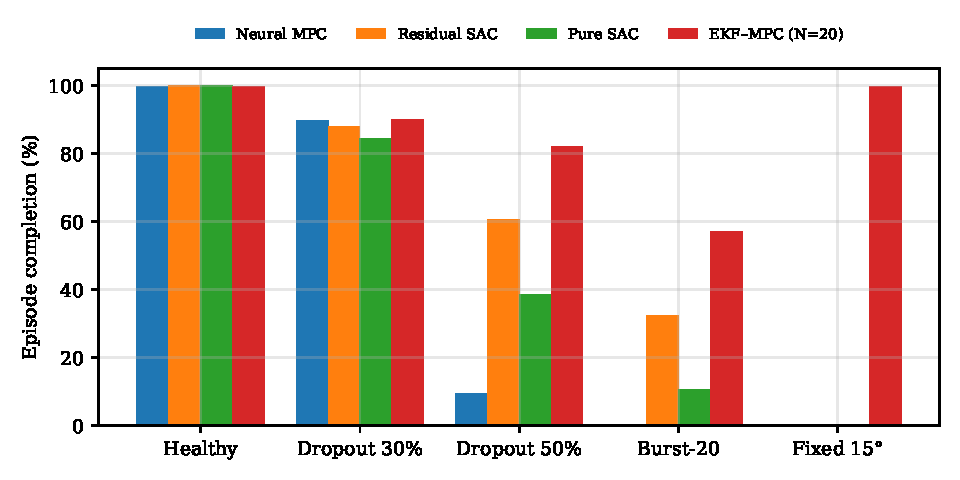
\includegraphics[width=.85\linewidth]{figs/fig3_focused.pdf}
\caption{Focused holdout episode completion by scenario (values of Table~\ref{tab:focus}).}\label{fig:focus}\end{figure}

\subsection{Sensitivity to prediction horizon}\label{sec:horizon}
Table~\ref{tab:hor} reports the EKF--MPC horizon sweep. Scenario-macro survival increases from 83.47\% ($N=10$) to 86.67\% ($N=40$). Survivor-conditioned tracking RMSE rises from 0.2310 to 0.2520\,rad, while mean episode control RMS falls from 2.3602 to 0.9438. Mean solver time increases monotonically with horizon, from \SI{6.85}{ms} to \SI{16.50}{ms}. It exceeded the \SI{10}{ms} sampling interval for $N=20,30,40$ in the first run (12.55, 15.25, 16.50\,ms) but only for $N=40$ in an identical repeat (10.62\,ms), so real-time schedulability is not established; solver times are an order of magnitude for this host, not a benchmark.

\begin{table}[t]\centering\small
\caption{EKF--MPC scenario-macro horizon sweep (1{,}500 unique episodes per horizon, first complete frozen run). RMSE is conditioned on survival. Solver calls: 630{,}685; 646{,}252; 651{,}961; 653{,}421 for $N=10,20,30,40$.}\label{tab:hor}
\resizebox{\linewidth}{!}{%
\begin{tabular}{rcccccc}\toprule
$N$ & Survival (\%) & Surv.\ RMSE (rad) & Control RMS & Solver time (ms) & Opt.\ inacc.\ (\% calls) & Failed calls\\\midrule
10 & 83.467 & 0.2310 & 2.3602 & 6.85 & 0.107 & 0\\
20 & 85.667 & 0.2346 & 1.6604 & 12.55 & 0.190 & 1\\
30 & 86.467 & 0.2453 & 1.1438 & 15.25 & 0.105 & 8\\
40 & 86.667 & 0.2520 & 0.9438 & 16.50 & 0.069 & 1\\\bottomrule
\end{tabular}}
\end{table}

Solves returning optimal inaccurate account for at most 0.19\% of calls at any horizon, and failed solves (executed as zero torque) occurred in 1, 8 and 1 steps at $N=20,30,40$ and none at $N=10$, each in a different episode; their effect on survival was not isolated.

\paragraph{Complete repeat.} The full run was repeated once with identical settings. The repeat reproduced all survival rates of Tables~\ref{tab:focus} and \ref{tab:horfault} exactly. For $N=20,30,40$ every deterministic per-episode metric was identical; only wall-clock quantities differed. At $N=10$ the continuous metrics of all 1{,}500 episodes differed (median absolute RMSE difference \num{9.6e-4}\,rad) and two episodes changed outcome (one lost, one gained), leaving macro survival unchanged at 83.467\%. Mean solver times were 36--46\% lower in the repeat (3.71, 7.55, 9.14 and 10.62\,ms), although code and tolerances were identical, so solver time depends strongly on host conditions.

\begin{table}[t]\centering\small
\caption{EKF--MPC survival (\%) by fault type and horizon (300 cases per cell).}\label{tab:horfault}
\begin{tabular}{lcccc}\toprule
Scenario & $N=10$ & $N=20$ & $N=30$ & $N=40$\\\midrule
Healthy & 98.00 & 99.67 & 100.00 & 100.00\\
Dropout 30\% & 87.33 & 90.00 & 91.00 & 91.33\\
Dropout 50\% & 79.33 & 82.00 & 84.00 & 84.33\\
Burst-20 & 54.67 & 57.00 & 57.33 & 57.67\\
Stuck roll $15^\circ$ & 98.00 & 99.67 & 100.00 & 100.00\\\bottomrule
\end{tabular}
\end{table}
\begin{figure}[t]\centering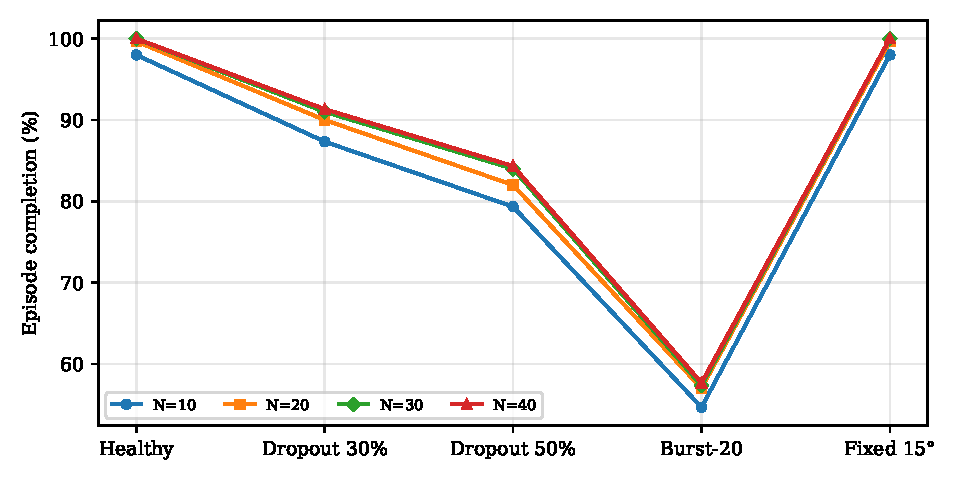
\includegraphics[width=.85\linewidth]{figs/fig4_horizon.pdf}
\caption{Effect of prediction horizon on EKF--MPC completion (Table~\ref{tab:horfault}); a plateau is apparent between $N=30$ and $N=40$.}\label{fig:hor}\end{figure}

The largest $N=20\to40$ improvement is at 50\% dropout (82.00\% versus 84.33\%; eight episodes rescued, one lost). Across 1{,}500 matched episodes, 17 are rescued by $N=40$ relative to $N=20$ and two experience the reverse, a net gain of 15 survivals (1.00 percentage point); this count is descriptive, not a hypothesis test. Burst-20 remains the hardest scenario (57.67\% at $N=40$), so a larger horizon alone is not a sufficient remedy for prolonged invalid measurements.

\subsection{Complementary 34-scenario benchmark}\label{sec:34}
A separate, previously recorded benchmark consists of 34 scenarios (healthy plant, 32 fault scenarios and one differential actuator-bias scenario), 100 evaluation seeds (77000--77099) per controller instance, one neural-MPC checkpoint (10-input network), one fixed-horizon residual-SAC checkpoint, five Pure SAC and five SAC+HOCBF (high-order control barrier function) policies at nominal rotor inertia: 40{,}800 controller--episode records. The HOCBF baseline is a SAC policy followed by a barrier-filter QP (class-$\mathcal K$ gains $\alpha_1=\alpha_2=2$, slack penalty $10^4$); it is a separate baseline, not the safety layer of the residual method. The Pure SAC and SAC+HOCBF policies were trained for 3{,}000{,}000 steps in eight parallel environments with a curriculum on initial roll amplitude (nine levels, up to $43.5^\circ$). Applied effort is the mean over episodes of $\sum\|\bm u\|_2^2$ divided by the episode length. This cohort has a different training-replication structure and is not pooled with Table~\ref{tab:focus}.

\begin{table}[t]\centering\small
\caption{Complementary 34-scenario benchmark (separate cohort). Effort is mean squared torque per step, not energy.}\label{tab:34}
\begin{tabular}{lcccc}\toprule
Controller & Survival (\%) & Surv.\ RMSE (rad) & Mean $\|\bm u\|_2^2$/step & Time (ms)\\\midrule
Neural MPC & 77.32 & 0.2043 & 28.56 & 0.0874\\
Residual SAC & 79.06 & 0.1229 & 58.61 & 0.3579\\
Pure SAC & 74.61 & 0.0877 & 672.40 & 0.2710\\
SAC+HOCBF & 67.01 & 0.1021 & 852.23 & 0.6517\\\bottomrule
\end{tabular}
\end{table}
\begin{figure}[t]\centering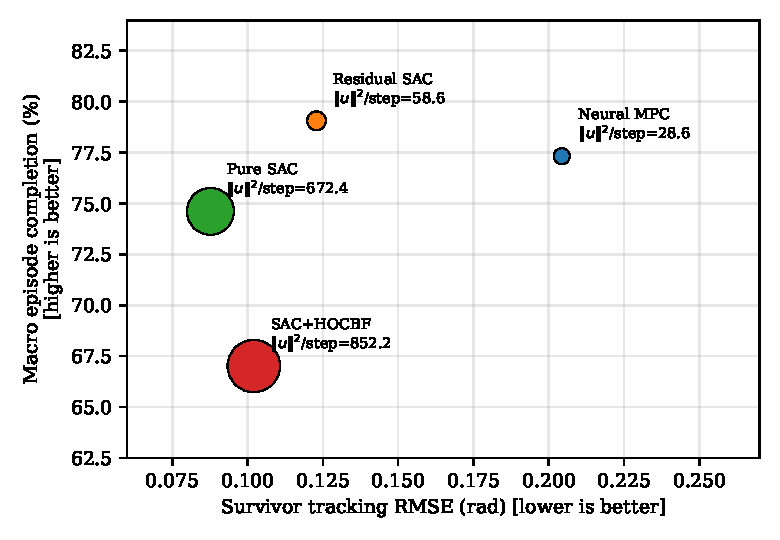
\includegraphics[width=.65\linewidth]{figs/fig5_tradeoff.pdf}
\caption{Survival--tracking--effort trade-off in the 34-scenario benchmark; marker area scales with mean squared torque per step; RMSE is conditional on survival.}\label{fig:trade}\end{figure}

The headline outcomes are not interchangeable: the residual checkpoint has the highest descriptive macro survival, Pure SAC the lowest survivor RMSE, and neural MPC the least squared torque. Low survivor RMSE does not imply robust crash avoidance. On the three aggregate axes (Fig.~\ref{fig:trade}) neural MPC, residual SAC and Pure SAC are non-dominated, whereas SAC+HOCBF is dominated by Pure SAC (a descriptive, not statistically certified, statement).

\paragraph{Paired inference.} Tables~\ref{tab:p1} and \ref{tab:p2} give pairwise survival and matched-survivor tracking contrasts (5{,}000 and 3{,}000 hierarchical bootstrap replicates, resampling scenarios, evaluation seeds and, for SAC families, training seeds; Holm correction over six comparisons). Five of six survival contrasts exclude zero; neural MPC versus Pure SAC is unresolved. Neural MPC and residual SAC are single checkpoints, so their intervals do not cover retraining variability. RMSE contrasts use only episodes in which both controllers survive, so they are neither a complete-scenario ranking nor equal to differences of marginal means in Table~\ref{tab:34}; statistical significance must not be mistaken for engineering relevance.

\begin{table}[t]\centering\small
\caption{Pairwise survival differences $\Delta S=S_A-S_B$ (percentage points), 95\% hierarchical bootstrap intervals, Holm-adjusted $p$.}\label{tab:p1}
\begin{tabular}{lccc}\toprule
$A-B$ & $\Delta S$ (pp) & 95\% CI (pp) & Holm $p$\\\midrule
Residual SAC $-$ Neural MPC & $+1.74$ & [0.44, 4.12] & $<0.001$\\
Neural MPC $-$ Pure SAC & $+2.72$ & [$-1.05$, 7.71] & 0.212\\
Neural MPC $-$ SAC+HOCBF & $+10.31$ & [3.21, 18.58] & 0.0036\\
Residual SAC $-$ Pure SAC & $+4.45$ & [0.62, 9.65] & 0.0312\\
Residual SAC $-$ SAC+HOCBF & $+12.05$ & [4.85, 20.68] & $<0.001$\\
Pure SAC $-$ SAC+HOCBF & $+7.59$ & [3.33, 12.74] & $<0.001$\\\bottomrule
\end{tabular}
\end{table}
\begin{table}[t]\centering\small
\caption{Paired tracking contrasts on jointly surviving episodes, $\Delta\mathrm{RMSE}=\mathrm{RMSE}_A-\mathrm{RMSE}_B$ (positive favors B). All six Holm-adjusted $p<0.002$.}\label{tab:p2}
\begin{tabular}{lccc}\toprule
$A-B$ & $\Delta$RMSE (rad) & 95\% CI (rad) & Joint-survivor scenarios\\\midrule
Neural MPC $-$ Residual SAC & $+0.0823$ & [0.0640, 0.0959] & 27/34\\
Neural MPC $-$ Pure SAC & $+0.1135$ & [0.0898, 0.1304] & 27/34\\
Neural MPC $-$ SAC+HOCBF & $+0.1157$ & [0.0960, 0.1284] & 27/34\\
Residual SAC $-$ Pure SAC & $+0.0319$ & [0.0274, 0.0357] & 28/34\\
Residual SAC $-$ SAC+HOCBF & $+0.0248$ & [0.0089, 0.0397] & 28/34\\
Pure SAC $-$ SAC+HOCBF & $-0.0182$ & [$-0.0226$, $-0.0140$] & 27/34\\\bottomrule
\end{tabular}
\end{table}

\paragraph{Where the differences arise.} The scenario-level rates (Appendix, Table~\ref{tab:app}) show that the aggregate ranking is carried by few scenarios. Six scenarios are failed by every controller: stuck roll measurement at $0^\circ$, $5^\circ$ and $15^\circ$ (from step 100), an actuator stuck at zero or at \SI{15}{N.m}, and an 8-step actuator delay. The residual advantage is concentrated in measurement-integrity and delay faults: burst-20 (35.0\% versus 0.0\% neural MPC, 15.8\% Pure SAC, 3.2\% SAC+HOCBF), 50\% dropout (95.0\% versus 90.0\%, 37.6\%, 27.8\%) and a 3-step actuator delay (96.0\% versus 94.0\%, 51.4\%, 0.2\%). Pure SAC falls to 75.0\% under 30\% actuator saturation and 83.6\% under 30\% dropout. SAC+HOCBF reaches only 60.8\% with a 50\% increase of rotor axial inertia (IwOmega $\times1.5$), where the other families are at 99--100\%. The effort difference reflects saturation: the mean fraction of steps with a torque channel at or above 99\% of $\tmax$ is 0.05\% (neural MPC), 0.12\% (residual SAC), 8.2\% (Pure SAC) and 12.4\% (SAC+HOCBF); the Pure SAC tracking advantage is thus obtained with near bang-bang torque and survivor-only RMSE.

\subsection{Sensitivity to CMG rotor axial-inertia reduction}\label{sec:inertia}
A separate sweep evaluates eight rotor axial-inertia scales with 100 seeds per controller instance (9{,}600 episodes). The plant $I_w$ is altered while the MPC model is unchanged, a genuine model-mismatch test. Table~\ref{tab:iw} and Fig.~\ref{fig:iw} show a sharp threshold in the neural MPC: survival falls from 0.98 at nominal inertia to 0.72 at 0.45, 0.34 at 0.42 and zero at 0.30. The residual keeps 0.95 down to 0.40 and 0.91 at 0.35 but drops to 0.71 at 0.30, whereas Pure SAC and SAC+HOCBF remain at or above 0.93. The controllers are those of Section~\ref{sec:34}; the adaptive-horizon policies are not part of this sweep.

\begin{table}[t]\centering\small
\caption{Survival probability versus rotor axial-inertia scale (100 seeds per controller instance; SAC families average five policies).}\label{tab:iw}
\begin{tabular}{ccccc}\toprule
$I_w$ scale & Neural MPC & Residual SAC & Pure SAC & SAC+HOCBF\\\midrule
1.00 & 0.980 & 0.990 & 1.000 & 0.996\\
0.60 & 0.950 & 0.980 & 0.990 & 0.986\\
0.50 & 0.890 & 0.970 & 0.990 & 0.982\\
0.45 & 0.720 & 0.950 & 0.990 & 0.980\\
0.42 & 0.340 & 0.950 & 0.990 & 0.968\\
0.40 & 0.190 & 0.950 & 0.980 & 0.966\\
0.35 & 0.040 & 0.910 & 0.978 & 0.962\\
0.30 & 0.000 & 0.710 & 0.976 & 0.938\\\bottomrule
\end{tabular}
\end{table}
\begin{figure}[t]\centering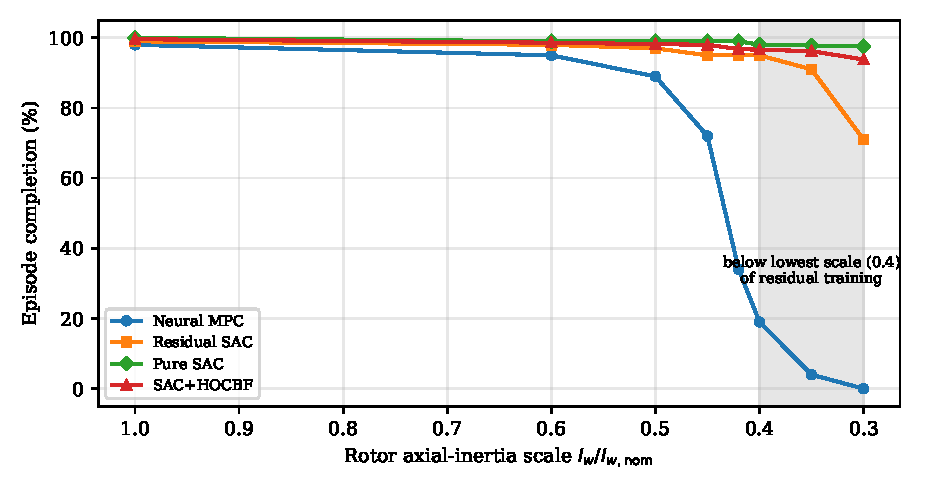
\includegraphics[width=.8\linewidth]{figs/fig6_inertia.pdf}
\caption{Survival versus rotor axial-inertia scale (values of Table~\ref{tab:iw}); the shaded region lies below the lowest scale (0.4) used to train the fixed-horizon residual.}\label{fig:iw}\end{figure}

Two caveats apply. The fixed-horizon residual was trained with sampled inertia variation (scales 1.0, 0.5, 0.45, 0.42, 0.4, chosen after pilot sweeps of the neural MPC where it fails), whereas the neural MPC was distilled from healthy-plant data only; scales 0.35 and 0.30 lie outside the residual's training range and 0.6 was not sampled. The SAC baselines were trained at nominal inertia (their logs mention no inertia variation), so the sweep does not compare equal training exposure and should not be generalized to other fault types. Two earlier sweeps with independent seeds point the same way: a neural-MPC sweep on seeds 73000--73099 gave survival 0.92, 0.73, 0.34, 0.13, 0.01, 0.00 at scales 0.50, 0.45, 0.42, 0.40, 0.35, 0.30, and a 30-episode screening of the online MPC showed graded degradation (0.97, 0.93, 0.80, 0.43, 0.00 at scales 1.0, 0.7, 0.6, 0.5, 0.4).

\subsection{Oracle-state barrier-filter diagnostic}
To test whether the weak SAC+HOCBF result is due to corrupted state information, the barrier filter was given either the measured or the true simulator state while the SAC policy still received the faulty observation (five scenarios, five HOCBF models, 100 paired seeds: 2{,}500 matched pairs). Table~\ref{tab:oracle} shows no clearly detectable improvement from true-state information (discordant pairs 10 versus 8 at IMU noise $7^\circ$ and 15 versus 20 at 50\% dropout; none elsewhere). This neither establishes equivalence nor identifies the cause of the HOCBF failures: the barrier condition uses an approximate discrete-time control influence, actuator faults let the applied torque depart from the QP command, and slack relaxation and solver fallback limit what nominal feasibility says about closed-loop safety. The oracle configuration is a diagnostic, not a deployable controller.

\begin{table}[t]\centering\small
\caption{Oracle-state minus measured-state HOCBF survival (paired; hierarchical bootstrap; McNemar $p$ pools discordant pairs and is exploratory).}\label{tab:oracle}
\begin{tabular}{lccc}\toprule
Scenario & Oracle $-$ measured (pp) & 95\% CI (pp) & McNemar $p$\\\midrule
Healthy & 0.0 & [0.0, 0.0] & 1.000\\
IMU noise $7^\circ$ & $+0.4$ & [$-1.6$, 2.4] & 0.815\\
IMU dropout 50\% & $-1.0$ & [$-3.8$, 1.8] & 0.500\\
Actuator saturation 30\% & 0.0 & [0.0, 0.0] & 1.000\\
Actuator delay 3 steps & 0.0 & [0.0, 0.0] & 1.000\\\bottomrule
\end{tabular}
\end{table}

\subsection{Estimator ablation and matched information}\label{sec:ablation}
To separate online optimization from the estimator, the online MPC ($N=20$, same weights, zero-torque fallback, seeds 78000--78099, 300 cases per scenario) was run in three information configurations: (i) raw, possibly corrupted roll measurements; (ii) a basic EKF with the noise settings of Section~\ref{sec:ekf} and the 9.21 innovation gate but without stale-data detection and covariance recovery; (iii) the robust EKF of the reported EKF--MPC runs, which adds both safeguards. In the paired check of Section~\ref{sec:ekf} the baseline mode reproduced configuration (ii) exactly, so (ii) and (iii) differ by the two safeguards together. Only survival and effort are compared across the three configurations; solver times are not.

\begin{table}[t]\centering\small
\caption{Survival (\%) of the online MPC ($N=20$) under three information configurations, with the neural MPC of Table~\ref{tab:focus} for reference (300 cases per cell).}\label{tab:abl}
\begin{tabular}{lcccc}\toprule
Scenario & (i) Raw & (ii) Gate-only EKF & (iii) Robust EKF & Neural MPC\\\midrule
Healthy & 99.67 & 99.67 & 99.67 & 99.67\\
Dropout 30\% & 84.67 & 50.33 & 90.00 & 89.67\\
Dropout 50\% & 1.00 & 1.67 & 82.00 & 9.33\\
Burst-20 & 0.00 & 0.00 & 57.00 & 0.00\\
Fixed roll $15^\circ$ & 0.00 & 62.67 & 99.67 & 0.00\\\midrule
Macro mean & 37.07 & 42.87 & 85.67 & 39.73\\\bottomrule
\end{tabular}
\end{table}

Without any estimator the online MPC completes only 1.00\% of the 50\%-dropout episodes and none under burst-20 or the fixed-angle fault, no better than the neural MPC; at 30\% dropout it reaches 84.67\%. The robust EKF raises these values to 82.00\%, 57.00\% and 99.67\%. A gate-only EKF is not sufficient: it helps with the fixed-angle fault (62.67\%) but lowers survival at 30\% dropout from 84.67\% to 50.33\% and leaves 50\% dropout (1.67\%) and burst-20 (0\%) unresolved; why it degrades 30\% dropout was not investigated. Paired by episode, the robust filter rescues 642 episodes that the gate-only version loses and loses none (119, 241, 171 and 111 at 30\% dropout, 50\% dropout, burst-20 and fixed angle). Without an estimator the optimizer is also stressed: 1{,}104 of 367{,}343 solver calls (0.30\%) failed and 2.22\% returned optimal inaccurate, against one failed call and 0.19\% with the robust EKF; mean episode $u_{\rm rms}$ was 6.56 (raw) against 1.58 and 1.66.

\paragraph{Neural MPC with the same gate-only EKF.} Table~\ref{tab:abl2} reports a later single run on the same 1{,}500 keys. In the EKF variants the six state channels of the controller input are replaced by the estimate and the roll error is recomputed from the estimated roll. With the same gate-only filter the neural and online MPC reach similar macro survival (44.07\% and 42.87\%) and neither resolves 50\% dropout or burst-20, supporting the reading that the safeguards of the robust estimator, not the controller class, carry the effect. The online-MPC rows differ slightly from Table~\ref{tab:abl} (outcomes differ in 4 and 56 of 1{,}500 episodes), consistent with the limited bitwise reproducibility of archived solver runs (Section~\ref{sec:limits}).

\begin{table}[t]\centering\small
\caption{Survival (\%) of four controllers in one run (seeds 78000--78099, $N=20$, 300 cases per scenario).}\label{tab:abl2}
\begin{tabular}{lccccc}\toprule
Controller & Healthy & Drop.\ 30\% & Drop.\ 50\% & Burst-20 & Fixed $15^\circ$\\\midrule
Online MPC, raw & 99.67 & 85.33 & 1.00 & 0.00 & 0.00\\
Online MPC + gate-only EKF & 99.67 & 51.00 & 2.33 & 0.00 & 61.33\\
Neural MPC, raw & 99.67 & 89.67 & 9.33 & 0.00 & 0.00\\
Neural MPC + gate-only EKF & 99.67 & 50.00 & 1.00 & 0.00 & 69.67\\\bottomrule
\end{tabular}
\end{table}

\paragraph{Matched information for all controllers.} Table~\ref{tab:match} evaluates the neural MPC, the five adaptive-horizon residual policies and the five Pure SAC policies on the keys of Table~\ref{tab:focus}, on raw measurements and with the robust EKF (combined mode, initialized from the first sample). In the EKF variants the six state channels are replaced by the estimate, the roll error is recomputed, and the previous-torque input is the applied torque; for the residual policies the base output and 15-dimensional observation are rebuilt from the estimate and the horizon channel remains free. The raw rows reproduce Table~\ref{tab:focus} exactly. With the robust EKF the neural MPC reaches 82.33\% and 56.67\% at 50\% dropout and burst-20, within 0.4 percentage points of EKF--MPC in every scenario (85.67\% mean for both); residual SAC reaches 81.00\% and 55.60\% (83.04\% mean) and Pure SAC 81.53\% and 53.00\% (80.11\% mean). The estimator raises the five-scenario mean by 45.9 points for the neural MPC, 26.8 for residual SAC and 33.4 for Pure SAC, and the ranking of Table~\ref{tab:focus} is lost: the residual's advantage over the neural MPC on raw measurements ($+16.5$ points) becomes a deficit of 2.6 points. The exception is the fixed-angle fault, where residual SAC and Pure SAC reach 89.40\% and 76.13\% against 99.67\% for neural MPC and EKF--MPC (not investigated). These are single runs on one seed cohort, with an estimator that has the exact plant model and a noise-free sensor, and the learned policies were not trained on estimator outputs.

\begin{table}[t]\centering\small
\caption{Survival (\%) with matched information (300 cases per scenario and policy; residual and Pure SAC aggregate five policies each). The last row is the EKF--MPC of Table~\ref{tab:focus}.}\label{tab:match}
\resizebox{\linewidth}{!}{%
\begin{tabular}{lcccccc}\toprule
Controller & Healthy & Drop.\ 30\% & Drop.\ 50\% & Burst-20 & Fixed $15^\circ$ & Mean\\\midrule
Neural MPC, raw & 99.67 & 89.67 & 9.33 & 0.00 & 0.00 & 39.73\\
Neural MPC + robust EKF & 99.67 & 90.00 & 82.33 & 56.67 & 99.67 & 85.67\\
Residual SAC, raw & 100.00 & 88.07 & 60.73 & 32.27 & 0.00 & 56.21\\
Residual SAC + robust EKF & 100.00 & 89.20 & 81.00 & 55.60 & 89.40 & 83.04\\
Pure SAC, raw & 100.00 & 84.27 & 38.53 & 10.73 & 0.00 & 46.71\\
Pure SAC + robust EKF & 100.00 & 89.87 & 81.53 & 53.00 & 76.13 & 80.11\\
Online MPC + robust EKF & 99.67 & 90.00 & 82.00 & 57.00 & 99.67 & 85.67\\\bottomrule
\end{tabular}}
\end{table}

Three conclusions are supported. First, online optimization alone does not explain the advantage of EKF--MPC over the learned policies. Second, the benefit depends on the stale-data and covariance-recovery logic rather than on filtering as such. Third, because the two safeguards were added together, their individual contributions are not separated. In the fixed-angle scenario the roll channel is rejected for roughly 400 steps after the onset at step 100 and the robust filter's roll estimate stays within \SI{2.5}{mrad} RMS of the true roll; since the plant equals the filter model and the healthy sensor is noise-free, this characterizes the stale-data logic under an exact model, not model mismatch (a supplementary test with noise and mismatch follows in Section~\ref{sec:noisemis}).

\subsection{Estimator sensitivity under sensor noise and rotor-inertia mismatch}\label{sec:noisemis}
In the focused scenarios the filter has the exact plant model and the healthy sensor is noise-free. To probe how much the conclusions of Section~\ref{sec:ablation} depend on these assumptions, a supplementary run compares four controllers under two conditions on identical seeds (300 episodes per cell). In the \emph{ideal} condition the plant equals the model and the sensor is noise-free. In the \emph{noise + mismatch} condition zero-mean Gaussian noise with standard deviations $(0.01,\,0.1,\,0.005,\,0.005,\,0.05,\,0.05)$ on the six measured channels $(\phi,\dot\phi,\delta_f,\delta_r,\dot\delta_f,\dot\delta_r)$ is added and the rotor axial inertia of the plant is reduced to $I_w=0.8\,I_{w,\rm nom}$ (20\% below nominal), while the model used by the EKF and by the MPC keeps the nominal $I_w$. No sensor fault is injected. The injected noise levels equal the values $\sigma_R$ of the filter's measurement-noise model (Section~\ref{sec:ekf}), whose settings are unchanged, so the noise itself is correctly modeled by the filter and the only mismatch is in the plant dynamics. Neural MPC, online MPC and the adaptive residual SAC receive the measurements directly, whereas EKF--MPC receives the estimator output. Besides survival and survivor-conditioned roll RMSE, the table reports the number of roll-channel samples rejected by the innovation gate and the roll-angle estimation error of the EKF.

\begin{table}[t]\centering\small
\caption{Supplementary stress test (300 episodes per cell, identical seeds). RMSE is the roll-tracking error conditioned on survival; EKF columns apply to EKF--MPC only (``--'': no estimator). Rejections are the total number of roll-channel samples rejected by the $\chi^2$ gate.}\label{tab:noisemis}
\begin{tabular}{llcccc}\toprule
Condition & Controller & Survival (\%) & RMSE (rad) & EKF rejections & EKF roll error (rad)\\\midrule
Ideal & Neural MPC & 100.0 & 0.216 & -- & --\\
Ideal & Online MPC & 100.0 & 0.217 & -- & --\\
Ideal & EKF--MPC & 100.0 & 0.217 & 0 & $\approx 0$\\
Ideal & Residual SAC (adaptive) & 100.0 & 0.088 & -- & --\\\midrule
Noise + mismatch ($I_w$) & Neural MPC & 97.3 & 0.237 & -- & --\\
Noise + mismatch ($I_w$) & Online MPC & 97.3 & 0.238 & -- & --\\
Noise + mismatch ($I_w$) & EKF--MPC & 84.0 & 0.253 & 4{,}173 & 0.077\\
Noise + mismatch ($I_w$) & Residual SAC (adaptive) & 99.7 & 0.091 & -- & --\\\bottomrule
\end{tabular}
\end{table}

In the ideal condition all four controllers complete every episode and the three MPC-based controllers track equally (0.216--0.217\,rad); the residual policy has a lower tracking error (0.088\,rad). Under noise and mismatch, the neural and online MPC on raw measurements lose little (97.3\% each, 292 of 300 episodes), and the residual SAC loses almost nothing (99.7\%, 299 of 300 episodes, 0.091\,rad). EKF--MPC is affected most: its completion falls to 84.0\% (252 of 300 episodes), its tracking error rises to 0.253\,rad, the gate rejects 4{,}173 roll samples (none in the ideal condition), and the roll-angle estimation error grows from approximately zero to 0.077\,rad (about $4.4^\circ$). The estimator that carried the advantage in the focused scenarios thus becomes the least robust component once its model and noise assumptions are violated.

Because the injected noise equals the filter's own noise model, the loss of EKF--MPC is most plausibly caused by the 20\% inertia mismatch rather than by the noise: the filter predicts a gyroscopic roll torque larger than the plant delivers, its roll prediction drifts from the true roll, and the resulting innovations exceed what the $\chi^2$ gate expects, so valid samples are discarded and the roll estimate becomes biased, which the MPC then uses. This mechanism is consistent with the counts above but was not isolated: no noise-only or mismatch-only run was made, and no run with re-tuned or adaptive noise covariances~\cite{mehra1970identification} or process noise inflated to cover the model error was made. The result therefore shows the sensitivity of this fixed-setting EKF, not of estimation in general. The comparison with the residual policy is further confounded by training exposure, since the residual was trained over a range of rotor-inertia scales (Section~\ref{sec:inertia}). It is a single run with one noise level and one mismatch level.

\subsection{Torque residual and horizon channel}\label{sec:lambda}
To separate the two outputs of the adaptive residual, the five policies were evaluated on the cohort of Table~\ref{tab:focus} (raw measurements; 7{,}500 episodes per row) with $\lambda\in\{0,5\}\Nm$ and the horizon chosen by the policy or frozen at $N=20$ (the frozen value also replaces the horizon index in the observation). Table~\ref{tab:lam} gives the result. With $\lambda=0$, $N=20$ the wrapper reproduces the neural MPC exactly in every cell. The torque residual alone raises the macro mean from 39.73\% to 53.93\% ($+14.2$ points), the horizon channel alone to 41.31\% ($+1.6$) and both to 56.21\% ($+16.5$); adding the horizon channel to the torque residual contributes 2.3 points, mostly at 50\% dropout (55.40\% to 60.73\%) and burst-20 (28.73\% to 32.27\%), and it recovers the small losses the torque residual alone causes at 30\% dropout and in the healthy scenario. The residual's gain on raw measurements is therefore mostly due to its torque correction. The policies were trained with a free horizon, so frozen-horizon rows are off-distribution and are lower bounds for policies trained with a fixed horizon.

\begin{table}[t]\centering\small
\caption{Survival (\%) of the adaptive-horizon residual with torque scale $\lambda$ and horizon varied (five policies, raw measurements).}\label{tab:lam}
\resizebox{\linewidth}{!}{%
\begin{tabular}{lcccccc}\toprule
Configuration & Healthy & Drop.\ 30\% & Drop.\ 50\% & Burst-20 & Fixed $15^\circ$ & Mean\\\midrule
Neural MPC (13-input, $N=20$) & 99.67 & 89.67 & 9.33 & 0.00 & 0.00 & 39.73\\
Residual, $\lambda=0$, $N=20$ & 99.67 & 89.67 & 9.33 & 0.00 & 0.00 & 39.73\\
Residual, $\lambda=0$, horizon free & 99.93 & 89.13 & 17.27 & 0.20 & 0.00 & 41.31\\
Residual, $\lambda=5$, $N=20$ & 99.20 & 86.33 & 55.40 & 28.73 & 0.00 & 53.93\\
Residual, $\lambda=5$, horizon free & 100.00 & 88.07 & 60.73 & 32.27 & 0.00 & 56.21\\\bottomrule
\end{tabular}}
\end{table}

%==============================================================
\section{Cross-simulator validation and frozen-controller transfer}\label{sec:cross}
\subsection{Protocol and model distinction}
A separate cross-simulator study tests whether reduced-model performance carries over to a higher-fidelity CMG model without retraining. Two checkpoints were held frozen: a Pure SAC policy (best-score checkpoint of seed 22, 620{,}000 of 1{,}000{,}000 steps) and an adaptive-horizon residual SAC policy (final checkpoint of seed 202, a 300{,}000-step run continued to 1{,}000{,}000 steps) whose base is the 13-input network. The checkpoints are selected differently (best-score versus final) and the training budgets are unequal, so this is not a compute-matched comparison. The evaluation seeds 500000--500004 are distinct from the earlier intervention-selection sweep, so no intervention parameter was chosen on them. For each controller and configuration, 30 supported fault scenarios were crossed with three buckets and five seeds (450 episodes), each lasting at most 500 steps with a $45^\circ$ survival threshold. Four parameter-fault scenarios of the 34-scenario suite were excluded because the MuJoCo wrapper does not implement them. Seeds, initial conditions, noise and fault generators were identical across configurations, enabling paired within-policy comparisons. Four configurations were compared:
\begin{itemize}
\item \textbf{Reduced}: the reduced equations integrated through the evaluation harness (reference);
\item \textbf{HF-A}: a more physically coupled MuJoCo model with two spinning flywheels, in which MuJoCo computes the gyroscopic coupling including the $\cos\delta$ dependence of the roll torque;
\item \textbf{Stop B}: HF-A with a damped physical joint stop on both gimbals at $\pm0.8$ rad;
\item \textbf{Supervisor C}: HF-A plus a software layer that scales down, linearly from 1 at $|\delta|=0.3$ rad to 0 at $|\delta|=0.5$ rad, the torque components pushing a gimbal further from zero (it never reverses or amplifies a command); it is not a formally enforced hard constraint.
\end{itemize}
Only HF-A represents unmodified zero-shot transfer. B modifies the plant and C the controller loop while keeping the trained weights unchanged; they demonstrate partial recovery by engineering changes, not unchanged zero-shot performance.

\paragraph{Model audit of HF-A.} A separate audit of the full-mode plant (diagnostics, not physical validation) agrees with the reduced equations where it should: gravity-only roll acceleration \SI{1.95873}{rad.s^{-2}} (reference 1.95873); roll acceleration $-4.70588$\,rad\,s$^{-2}$ for a front-gimbal rate of 1\,rad\,s$^{-1}$ and $+4.70588$ for the rear, $-9.41176$ for the differential case and zero for the common mode; no coupling when the rotors are at rest; and a gimbal acceleration of 100.0004\,rad\,s$^{-2}$ for a \SI{10}{N.m} command (reference 100), obtained with an actuator gear ratio of about 2.5. Flywheel speeds are re-initialized to $\pm\Omega$ at every outer step, the roll axis is a constrained ground hinge without contact, and the mass and center-of-mass compensation is an effective calibration. The reduced MuJoCo mode passes three plant checks: the one-step error against a 100-times-finer RK4 integration has mean \num{1.4e-6} and maximum \num{4.9e-6}\,rad (project RK4: \num{1.1e-6} and \num{6.9e-6}), the step is stateless and deterministic, and a state-feedback LQR acting on the measured state yields identical per-episode survival on both plants (20 episodes per scenario; mean absolute RMSE difference at most \num{9.2e-7}\,rad). Two differences from the reduced plant that Eq.~\eqref{eq:gimbal} does not contain appear in the full mode: in an open-loop test from $\phi_0=0.05$ rad with zero torque the reduced plant leaves the $45^\circ$ threshold within one second ($\phi=0.816$ rad) whereas HF-A remains at 0.051 rad; and the gimbal rate after one step of a \SI{10}{N.m} command is 3.1\% lower in HF-A (0.960 versus 0.990 rad/s). Both are consistent with a gyroscopic reaction on the gimbal axis absent from the reduced model, i.e.\ a second model difference besides the $\cos\delta$ dependence; the mechanism was not isolated.

\subsection{Survival degradation and intervention response}
Table~\ref{tab:xs} and Fig.~\ref{fig:xs} show the confirmatory counts. Pure SAC decreases from 325/450 (72.2\%) in Reduced to 77/450 (17.1\%) in HF-A; residual SAC from 339/450 (75.3\%) to 14/450 (3.1\%). The ordering observed in Reduced thus reverses in unmodified HF-A. Stop B improves residual survival to 180/450 (40.0\%) and Supervisor C to 196/450 (43.6\%); both leave a substantial gap to Reduced, and for Pure SAC the gains are considerably smaller.

\begin{table}[t]\centering\small
\caption{Confirmatory cross-simulator survival on seeds 500000--500004 (450 paired keys per controller/configuration; 95\% Wilson intervals). Only HF-A is unmodified zero-shot transfer. Scenarios share seeds and initial conditions, so the intervals are optimistic.}\label{tab:xs}
\begin{tabular}{lcc}\toprule
Configuration & Pure SAC & Residual SAC + neural MPC\\\midrule
Reduced (reference) & 325/450 (72.2\%) [67.9, 76.2] & 339/450 (75.3\%) [71.1, 79.1]\\
HF-A (unmodified transfer) & 77/450 (17.1\%) [13.9, 20.9] & 14/450 (3.1\%) [1.9, 5.2]\\
Stop B ($\pm0.8$ rad) & 91/450 (20.2\%) [16.8, 24.2] & 180/450 (40.0\%) [35.6, 44.6]\\
Supervisor C & 88/450 (19.6\%) [16.2, 23.5] & 196/450 (43.6\%) [39.0, 48.2]\\\bottomrule
\end{tabular}
\end{table}
\begin{figure}[t]\centering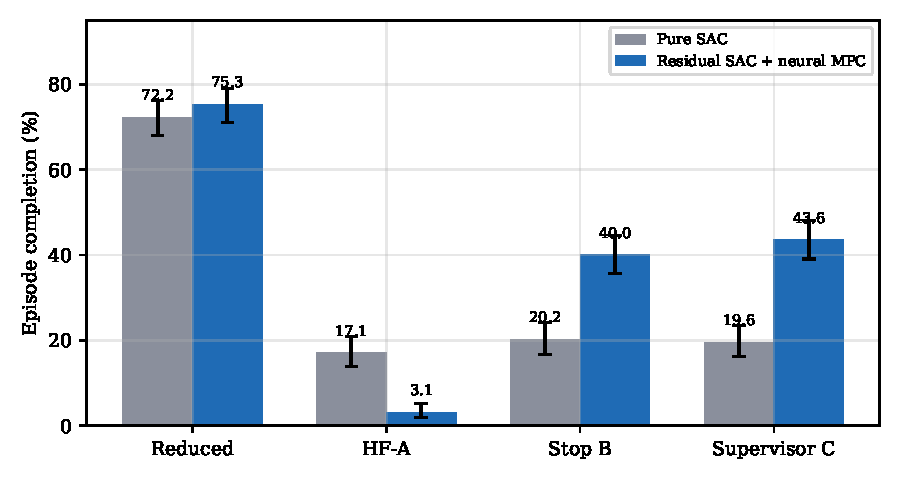
\includegraphics[width=.8\linewidth]{figs/fig7_crosssim.pdf}
\caption{Held-out cross-simulator episode completion of frozen policies (error bars: 95\% Wilson intervals; values of Table~\ref{tab:xs}). A distinct 30-scenario experiment, not pooled with the five-scenario EKF study.}\label{fig:xs}\end{figure}

A state-feedback LQR (discrete-time, $Q=\mathrm{diag}(100,10,20,20,1,1)$, $R=0.1I_2$, from the nominal model linearized at $\phi=0$ and applied to the measured state) stabilized the HF-A model in 40/40 episodes in each of two scenarios (healthy sensor and 30\% roll dropout; initial roll uniform in $\pm0.3$ rad, roll rate in $\pm0.8$ rad/s, 500 steps). The largest gimbal angle over all episodes was 0.518 and 0.501 rad, below 0.6 rad (on the reduced plant 0.263 and 0.329 rad, also 40/40). The same gains fail under the fixed $15^\circ$ measurement (0/20), as expected without fault handling. Stabilization is therefore achievable for the tested configurations with gimbal angles well below $\pm\pi/2$, although the LQR needs larger gimbal angles in HF-A than on the reduced plant; this does not establish global controllability or exclude other causes of the policies' failures.

\subsection{Paired comparisons and cluster-aware uncertainty}
Table~\ref{tab:disc} tabulates discordant paired episodes. Comparing Reduced, Stop B and Supervisor C with HF-A gives 257, 39 and 36 intervention-only survivors versus 9, 25 and 25 HF-A-only survivors for Pure SAC; for residual SAC the counts are 328 versus 3, 166 versus 0 and 182 versus 0. Episode-level sign tests are descriptive because seeds and buckets recur across scenarios. A conservative complementary analysis resamples the independent evaluation seed as the cluster: each of five clusters contains 90 paired keys per controller, and all $5^5=3125$ ordered with-replacement samples were enumerated exactly (Table~\ref{tab:boot}). The small number of clusters still limits coverage reliability and does not capture retraining or new-scenario variability.

\begin{table}[t]\centering\small
\caption{Paired comparisons against HF-A (episodes surviving in only one configuration); sign-test $p$ values are descriptive.}\label{tab:disc}
\begin{tabular}{llccc}\toprule
Comparison & Controller & Only in HF-A & Only in intervention & Sign-test $p$\\\midrule
B vs A & Residual SAC & 0 & 166 & $2\times10^{-50}$\\
B vs A & Pure SAC & 25 & 39 & 0.10\\
C vs A & Residual SAC & 0 & 182 & $3\times10^{-55}$\\
C vs A & Pure SAC & 25 & 36 & 0.20\\\bottomrule
\end{tabular}
\end{table}
\begin{table}[t]\centering\small
\caption{Seed-cluster bootstrap survival contrasts relative to unmodified HF-A (percentage points; five evaluation-seed clusters within the fixed 30-scenario suite).}\label{tab:boot}
\begin{tabular}{llcc}\toprule
Controller & Comparison $-$ HF-A & Difference (pp) & 95\% CI (pp)\\\midrule
Pure SAC & Reduced & $+55.1$ & [$+25.3$, $+73.8$]\\
Pure SAC & Stop B & $+3.1$ & [$-7.8$, $+19.3$]\\
Pure SAC & Supervisor C & $+2.4$ & [$-7.8$, $+17.3$]\\
Residual SAC & Reduced & $+72.2$ & [$+67.6$, $+76.0$]\\
Residual SAC & Stop B & $+36.9$ & [$+11.8$, $+62.0$]\\
Residual SAC & Supervisor C & $+40.4$ & [$+12.4$, $+68.4$]\\\bottomrule
\end{tabular}
\end{table}

\subsection{Fault-family results}
Table~\ref{tab:fam} breaks the survival down by fault family. Stuck-sensor and stuck-actuator scenarios also fail in Reduced, so these failures belong to the controllers and not to the higher-fidelity physics. The largest residual-SAC recoveries with stop or supervisor occur for healthy operation, IMU noise, dropout, actuator bias and saturation, whereas Pure SAC remains largely unchanged. Because each family aggregates few scenarios, individual cells are noisy. The actuator-fault families are evaluated in a harness whose plant receives the clipped faulted torque, which differs from the 34-scenario harness (Section~\ref{sec:limits}).

\begin{table}[t]\centering\small
\caption{Survival rate by fault family on the confirmatory seeds (P = Pure SAC, R = Residual SAC); 15 episodes per scenario (three buckets $\times$ five seeds); Healthy is a single scenario.}\label{tab:fam}
\resizebox{\linewidth}{!}{%
\begin{tabular}{lcccc}\toprule
Fault family & Reduced P / R & HF-A P / R & Stop 0.8 P / R & Supervisor P / R\\\midrule
Healthy & 1.00 / 1.00 & 0.27 / 0.07 & 0.27 / 0.60 & 0.27 / 0.53\\
IMU noise & 1.00 / 0.93 & 0.20 / 0.02 & 0.22 / 0.53 & 0.16 / 0.49\\
IMU roll bias & 1.00 / 1.00 & 0.16 / 0.00 & 0.11 / 0.20 & 0.13 / 0.40\\
IMU drift & 1.00 / 1.00 & 0.27 / 0.07 & 0.13 / 0.30 & 0.20 / 0.50\\
IMU dropout & 0.87 / 0.93 & 0.24 / 0.07 & 0.27 / 0.60 & 0.27 / 0.49\\
Intermittent IMU & 0.43 / 0.63 & 0.10 / 0.00 & 0.27 / 0.50 & 0.23 / 0.47\\
Stuck roll sensor & 0.00 / 0.00 & 0.00 / 0.00 & 0.00 / 0.09 & 0.00 / 0.07\\
Combined faults & 1.00 / 0.93 & 0.20 / 0.00 & 0.13 / 0.20 & 0.13 / 0.60\\
Actuator bias & 1.00 / 1.00 & 0.27 / 0.00 & 0.27 / 0.60 & 0.27 / 0.53\\
Actuator saturation & 1.00 / 1.00 & 0.20 / 0.07 & 0.27 / 0.43 & 0.27 / 0.53\\
Actuator stuck & 0.00 / 0.00 & 0.07 / 0.10 & 0.17 / 0.23 & 0.20 / 0.20\\\bottomrule
\end{tabular}}
\end{table}

\subsection{Dynamics-based interpretation and design requirements}\label{sec:mech}
Equation~\eqref{eq:roll} contains $\dot\delta_f-\dot\delta_r$ but no explicit gimbal-angle reduction of gyroscopic roll authority; the roll torque depends on gimbal rates, not angles, so nothing in the reduced model penalizes a gimbal parked at $\pm90^\circ$. In the reduced plant both policies routinely reach the $\pm90^\circ$ limit: the maximum gimbal angle of an episode is at least 1.5 rad in 95.8\% (Pure SAC) and 96.9\% (residual SAC) of the 450 episodes, including every surviving episode, so reaching the limit is harmless there; over 30 surviving episodes per policy the larger gimbal angle is at least 1.55 rad in 92.5\% of the steps for Pure SAC and 86.8\% for residual SAC. The higher-fidelity geometry introduces an approximate $\cos\delta$ dependence of each gimbal's roll projection, besides other coupled dynamics: $\cos(1.0)\approx0.54$, $\cos(1.45)\approx0.12$, $\cos(1.55)\approx0.02$, so approaching $\pi/2$ can sharply reduce the available roll moment. In HF-A the maximum gimbal angle is at least 1.5 rad in 99.6\% (Pure SAC) and 99.3\% (residual SAC) of the episodes, survivors included (all 77 surviving Pure SAC episodes and 13 of 14 surviving residual episodes reach 1.4 rad), so the peak angle alone does not separate failures from survivors; time near the limit was not recorded. With Stop B the maximum angle never exceeds 0.99 rad (median 0.86 rad; 99.7\% of episodes touch 0.8 rad, i.e.\ the damped stop is overshot by up to about 0.19 rad) and residual survival rises from 3.1\% to 40.0\%. Under Supervisor C the gimbal still reaches 1.5 rad in 92.9\% (Pure SAC) and 88.4\% (residual SAC) of episodes, yet residual survival rises to 43.6\%; over the 900 episodes of C survival is 27.6\% in the 816 episodes whose maximum angle reaches 1.5 rad and 70.2\% in the 84 that stay below it. The supervisor therefore does not keep the gimbals away from the limit, its benefit cannot be attributed to avoiding the region near $\pm90^\circ$, and the data show an association with the peak angle, not a mechanism.

\begin{figure}[t]\centering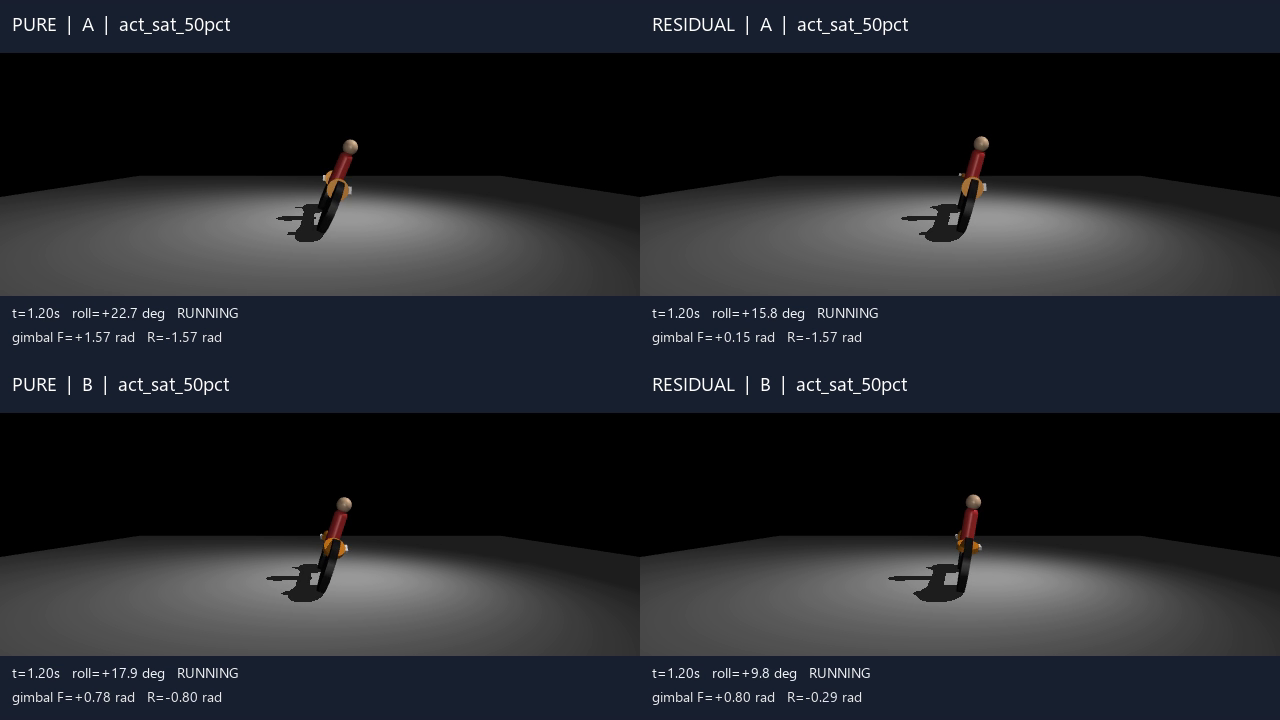
\includegraphics[width=.95\linewidth]{figs/fig8_mujoco_frames.png}
\caption{MuJoCo frames at $t=1.20$ s for the \texttt{act\_sat\_50pct} scenario, seed 500000, bucket 0 (rows: HF-A and Stop B; columns: Pure SAC and residual SAC). Roll / front gimbal / rear gimbal: Pure--A $+22.7^\circ$/$+1.57$/$-1.57$ rad; Residual--A $+15.8^\circ$/$+0.15$/$-1.57$ rad; Pure--B $+17.9^\circ$/$+0.78$/$-0.80$ rad; Residual--B $+9.8^\circ$/$+0.80$/$-0.29$ rad. All four episodes are still running at this instant and end in failure later (after 137, 194, 161 and 237 steps).}\label{fig:frames}\end{figure}

Figure~\ref{fig:frames} illustrates one actuator-saturation scenario at $t=1.20$ s. In HF-A both policies have at least one gimbal pinned at $\pm1.57$ rad, whereas the $\pm0.8$ rad stop keeps both gimbals at or below about 0.8 rad and yields smaller roll angles ($17.9^\circ$ Pure, $9.8^\circ$ Residual, versus $22.7^\circ$ and $15.8^\circ$ in A). This is a single frame, not a survival result.

\paragraph{Parameter selection.} An exploratory stop sweep (30 episodes per controller, healthy and 30\%-dropout cases) informed intervention selection. Because the 0.8-rad limit was selected on those seeds, its 30/30 residual survival is optimistic; on independent seeds residual survival was 40.0\% overall and 60\% in the healthy scenario. In the selection run (30 scenarios, seeds 400000--400002) residual SAC survived 188/270 episodes (69.6\%) with the 0.8-rad stop. In the sweep (seeds 400000--400004, two scenarios) the 0.3-rad stop yielded 0/30 Pure SAC and 6/30 residual SAC; the 0.8- and 1.1-rad stops yielded 18/30 and 17/30 for Pure SAC and 30/30 for residual SAC. These are parameter-selection results, not independent generalization estimates.

\paragraph{Design requirements.} A tight mechanical stop alters roll authority, collision impulses, dwell and torque transmission, so its benefit cannot be attributed solely to avoiding the near-singular region; Supervisor C does not prevent the gimbals from reaching the limit. Neither intervention isolates a unique mechanism or restores the reduced-model success rate, and Pure SAC does not benefit significantly from either (Tables~\ref{tab:disc}, \ref{tab:boot}), so its failures are not primarily explained by the gimbal singularity. The results nevertheless yield requirements for hardware deployment: (a) training models must include the angle-dependent CMG authority and a near-singularity cost; (b) gimbal stops or supervisors must be treated as part of the plant and controller that is validated, not as add-ons; (c) the second, gyroscopic-reaction model difference must be identified before transfer claims; (d) paired evaluation on new seeds must follow any intervention tuning.

%==============================================================
\section{Discussion}
Across the focused suite on raw measurements, estimator-aided online MPC is markedly less susceptible to frozen and missing roll measurements than the particular learned checkpoints. The matched-information runs (Table~\ref{tab:match}) show that this difference is carried by the information pathway: when the neural MPC receives the output of the same robust EKF it reproduces the survival of EKF--MPC within 0.4 percentage points in every scenario (85.67\% mean for both), and the residual and Pure SAC policies reach 83.04\% and 80.11\%. Online optimization is therefore not needed for the estimator-based advantage, and once information is matched the spread between controller classes is small; the fixed-angle scenario, where the learned policies lose 10 and 24 points against the neural MPC, is the exception. Conversely, without the estimator the same MPC completes 1.00\% of the 50\%-dropout episodes, and a gate-only EKF is not enough, so the stale-data and covariance-recovery safeguards carry the effect, although their individual contributions remain unseparated. At moderate (30\%) dropout the advantage largely disappears (90.00\% versus 89.67\%). The residual correction, which helps on raw measurements and owes most of its gain to the torque correction (Section~\ref{sec:lambda}), does not help once the estimator is present (83.04\% versus 85.67\%).

The advantage of the estimator is conditional on the accuracy of its model. In the supplementary stress test (Table~\ref{tab:noisemis}), combining sensor noise (matched to the filter's noise model) with a 20\% rotor-inertia reduction lowers EKF--MPC completion from 100\% to 84.0\% with 4{,}173 roll-channel rejections, while the raw-measurement neural and online MPC keep 97.3\% and the residual SAC 99.7\%. The matched-information result above therefore holds under an exact model and a noise-free sensor; once the filter's assumptions are violated, a fixed-setting EKF can be the weakest element of the loop. Two caveats limit the interpretation: because the noise equals the filter's own noise model the loss is most plausibly due to the inertia mismatch, but no noise-only or mismatch-only run separates the two, and the residual had seen a range of inertia scales during training.


A fixed $15^\circ$ sensor reading is not equivalent to a physical lean angle of $15^\circ$, and survival under this fault should not be described as physical balance recovery. The filter rejects the roll channel for the remaining steps and propagates its estimate with the nominal model, which here coincides with the plant; the high survival reflects accurate open-loop prediction over about four seconds under an exact model and a noise-free sensor, not robustness to model error.

Increasing the MPC horizon exhibits diminishing benefits: the gain from $N=30$ to $N=40$ is 0.20 percentage points on the macro measure, while survivor RMSE and solver time are larger for $N=40$ (0.2520 versus 0.2453\,rad; 16.50 versus 15.25\,ms). $N=30$ is thus a defensible compromise, not a formally optimized choice; the solver-time growth indicates computational cost but not real-time feasibility.

\paragraph{Long-duration behavior.}\label{sec:long}
To check that the five-second completion rates do not conceal delayed instability or a secular drift of the gimbals, a supplementary 30-second test (3{,}000 control steps at \SI{100}{\hertz}) was run on the nominal plant (seeds 620000--620001 across initial-condition buckets 0--2, i.e.\ six episodes per controller). The distilled neural MPC and EKF--MPC completed all 3{,}000 steps in every episode and kept the gimbals well inside the limit (maximum $|\delta|\le56.7^\circ$, a margin of more than $33^\circ$ to the $\pm90^\circ$ bound of the reduced model). The adaptive residual SAC also completed every episode, with the lowest tracking error (0.073\,rad RMSE), but its gimbal angle reached the $90.0^\circ$ bound. This is consistent with the tendency of the learned policies to park the gimbals where the roll authority of a $\cos\delta$ model vanishes (Section~\ref{sec:mech}) and with their loss of survival in the cross-simulator transfer (Section~\ref{sec:cross}); it is not a demonstration of that mechanism, since the reduced model has no angle dependence and the transfer gap has other candidate causes (Section~\ref{sec:mech}). The test covers the nominal plant and few episodes, so it can reveal delayed instability or gimbal drift but does not estimate long-horizon completion rates.

The cross-simulator test identifies a much stronger limitation than those evident in the reduced-order benchmarks: frozen learned policies can lose most of their survival margin under physically different CMG kinematics. The reduced model hides a physically important constraint because it omits the dependence of CMG torque on gimbal angle; controllers trained on it can learn to park the gimbals near the singularity, which is harmless there and fatal in the higher-fidelity model. Only the unmodified HF-A row tests direct zero-shot transfer. The stop and supervisor variants recover part of the residual-SAC loss but should not be credited as zero-shot success, and the remaining gap (40--44\% versus 75\%) shows that the singularity is not the only mismatch; the open-loop and gimbal-rate differences of Section~\ref{sec:cross} point to a gyroscopic reaction on the gimbal axis as a further candidate. The MuJoCo study uses five seed clusters rather than the 100-seed focused cohort, so percentage comparisons across suites are not controlled head-to-head rankings.

The 34-scenario benchmark underscores why selection cannot rest on a single metric: the low-RMSE Pure SAC trials are selected survivors, its actuation cost is much larger than that of neural MPC, and the largest average survival is attained by residual SAC. Comparison with the focused holdout requires caution because scenario distribution, training-replicate structure, residual family and checkpoint identities differ.

The distillation result is the least ambiguous component: on a healthy plant the neural policy reproduces the teacher's survival and tracking while cutting measured command-computation time by about two orders of magnitude. Its fidelity, however, is fidelity to the nominal teacher, and the inertia sweep shows that this also reproduces the teacher's sensitivity to plant mismatch (survival 0.34 at 42\% of nominal rotor inertia). The residual and SAC baselines remain far more robust, but the comparison is confounded by training exposure: the residual was trained on the very range of scales in which the neural MPC fails, so the sweep supports the use of a residual correction for robustness without isolating how much of the benefit stems from that targeted exposure.

%==============================================================
\section{Limitations and reproducibility}\label{sec:limits}
\paragraph{Scope.} All evidence is simulation-based; no hardware-in-the-loop test, motorcycle experiment or formal stability guarantee is presented. The reduced model omits tire--road contact and actuator internal dynamics, and injected faults affect only the roll-angle/rate channels. In the focused EKF scenarios the filter uses the exact nominal plant model and the healthy sensor is noise-free, so these estimator results do not characterize robustness to model error or sensor noise. Only one supplementary condition combining sensor noise with rotor-inertia mismatch was tested (Section~\ref{sec:noisemis}); it did not separate the two effects (the injected noise equals the filter's noise model, which points to the inertia mismatch), did not re-tune the filter, and showed a marked loss for EKF--MPC. The learned policies were not trained on estimator outputs, noise or mismatch. The MuJoCo model does not reproduce complete riding dynamics (contact-rich forward motion, steering); rotor spin is prescribed at the start of each control step, and actuator gearing is calibrated so that gimbal acceleration matches the reduced model. Gimbal stops and supervisory torque limiting alter the plant or loop and are not unmodified zero-shot transfer. Five-second completion rates do not establish persistent stabilization; a supplementary 30-second test on the nominal plant (Section~\ref{sec:long}) found no delayed instability for the neural MPC and EKF--MPC, but it covers one nominal condition with few episodes, and fault, noise and mismatch conditions were not run over long horizons. Survivor-conditioned RMSE cannot be generalized to failed trajectories. Solver times are single-host means, not worst-case guarantees. The focused comparisons use a limited number of independently trained checkpoints (neural MPC, the 34-scenario residual and EKF--MPC are single configurations), and the adaptive residual policies were trained with unequal budgets. The cross-simulator study uses five seed clusters and 30 supported scenarios and does not cover retraining. An ablation separating the two EKF safeguards, and an intermediate plant isolating $\cos\delta$ from other coupling differences, were not performed. The code defining the Stop~B and Supervisor~C variants is specified here by the parameters of Section~\ref{sec:cross}; its release with the archive is pending.

\paragraph{Harness semantics.} The 34-scenario benchmark applies the faulted torque to the plant before clipping it to $\pm\SI{50}{N.m}$ (a gain of 1.3 or an added bias can therefore exceed 50\,N\,m, while logged effort uses the clipped value), whereas the focused-holdout and MuJoCo harness applies the clipped torque. They coincide for sensor faults but not actuator faults, so the actuator-fault results of Tables~\ref{tab:fam} and \ref{tab:app} are not computed under identical semantics.

\paragraph{Reproducibility of the EKF--MPC runs.} The horizon study was regenerated in a single complete run of 6{,}000 episodes and supersedes all earlier EKF--MPC results. Its complete repeat reproduced survival at every horizon and scenario, deterministic per-episode metrics at $N=20,30,40$, and differed at $N=10$ in two outcomes and in all continuous metrics (solver times differed by 36--46\%). On subsets, a re-run at $N=20$ (seeds 78000--78009, 150 episodes) against an earlier archived run reproduced survival and step counts but not continuous metrics (median absolute RMSE difference about \num{5e-4}\,rad, maximum \num{8.4e-3}\,rad; median $u_{\rm rms}$ difference about \num{8e-3}\,N\,m, maximum 1.16\,N\,m; 36 episodes differed in EKF rejection count). Over all 1{,}500 episodes the earlier archived run differs from the final one in two outcomes. A repeat of the gate-only online-MPC run on seeds 78000--78009 differed from its archived counterpart in 4 survival outcomes and 33 step counts of 150, so Table~\ref{tab:abl} (i) and (ii) are single archived runs whose survival is not bitwise reproducible, though the differences are small relative to the effects discussed. Survival is therefore the more robust outcome; the source of the variation was not identified (solver warm-start state carried across episodes is one untested candidate). A small fraction of solver calls returned optimal inaccurate (0.07--0.19\%) or failed (0, 1, 8, 1 calls at $N=10,20,30,40$ in the first run); failed solves were executed as zero torque.

\paragraph{Computing environment.} All experiments ran on one x86-64 workstation (8 cores, Windows~11) with Python 3.10, NumPy 1.26.4, CVXPY 1.4.3, OSQP 0.6.6, PyTorch 2.6.0, Stable-Baselines3 2.3.2 and MuJoCo 3.16.0. Reported timings are single-thread CPU timings; some network training used a GPU. The residual checkpoints of seeds 404 and 505 were converted from NumPy~2 to NumPy~1.26; converted actor outputs agreed with the originals within $10^{-6}$ on 100 probe observations (a numerical, not closed-loop, equivalence check).

%==============================================================
\section{Conclusions}
In the examined motorcycle--CMG simulation, severe roll-measurement failures are overcome by the information pathway rather than by online optimization: on raw measurements the distilled neural MPC fails, while with the same robust EKF it matches EKF--MPC. At $N=20$, robust EKF--MPC yields 82.00\% survival under 50\% dropout and 57.00\% under 20-step intermittent corruption, versus 60.73\% and 32.27\% for residual SAC. Removing the estimator reduces survival at 50\% dropout to 1.00\% (0.00\% under burst-20), and a gate-only EKF does not recover it (1.67\%), so the stale-data and covariance-recovery safeguards, not online optimization, account for the advantage. With the same robust EKF the neural MPC, residual SAC and Pure SAC reach 85.67\%, 83.04\% and 80.11\% five-scenario survival (EKF--MPC 85.67\%), and the residual's gain on raw measurements is carried mostly by its torque correction rather than the horizon channel. The estimator advantage is conditional on an accurate filter model: with sensor noise matched to the filter's model and a 20\% rotor-inertia reduction applied together, EKF--MPC survival falls from 100\% to 84.0\% (4{,}173 rejected roll samples), against 97.3\% for the neural and online MPC and 99.7\% for residual SAC on raw measurements. Increasing the horizon from 10 to 40 improves macro survival from 83.47\% to 86.67\% but increases solver time (6.85 to 16.50\,ms; 3.71 to 10.62\,ms in an identical repeat) and survivor RMSE (0.2310 to 0.2520\,rad). The 34-scenario benchmark shows a distinct trade-off in which residual SAC achieves the best average survival while Pure SAC and neural MPC favor conditional tracking error and control effort, respectively. The cross-simulator experiment reveals deployment sensitivity: residual SAC survival falls from 75.3\% to 3.1\% on unmodified HF-A and rises to 40.0\% and 43.6\% with damped gimbal stops and command supervision, which mitigate but do not close the gap and are not unchanged zero-shot transfer. In a supplementary 30-second nominal-plant test the neural MPC and EKF--MPC remained stable with gimbal angles below $56.7^\circ$, whereas the residual SAC, despite the lowest tracking error, drove the gimbals to the $90^\circ$ bound. The distilled neural MPC matches its teacher's healthy-plant survival at about $1/181$ of the computation time but inherits its fragility under rotor-inertia reduction, which the residual correction, trained on that range, largely removes in the tested sweep.

Future work should include physics-aware training with angle-dependent CMG authority and a near-singularity cost (retraining neural MPC and SAC on a model with $\cos\delta$, followed by the same paired protocol on new seeds), diagnosis of the gyroscopic-reaction mismatch, explicit real-time feasibility studies, longer-duration tests, training the learned policies on estimator outputs, noise and model mismatch, re-tuned or adaptive-covariance estimators under mismatch with noise and mismatch separated, and more independent training replications. All conclusions remain conditional on the evaluated simulation models.

%==============================================================
\section*{Declaration of competing interest}
\todo{State competing interests, or: The authors declare that they have no known competing financial interests or personal relationships that could have appeared to influence the work reported in this paper.}

\section*{Funding}
\todo{Funding statement.}

\section*{CRediT authorship contribution statement}
\todo{Author contributions using CRediT roles.}

\section*{Data availability}
The simulation models, trained network weights, and episode-level datasets generated during this study are available from the corresponding author upon reasonable request.

\section*{Declaration of generative AI use}
\todo{Complete according to Elsevier's policy on generative AI in the writing process.}

%==============================================================
\appendix
\section{Scenario-level survival in the 34-scenario benchmark}
Table~\ref{tab:app} lists survival (\%) per scenario (100 seeds per instance; SAC families average five policies), sorted by the residual SAC rate. \texttt{param\_iw\_p50} is a 50\% increase of the rotor axial inertia ($I_w\Omega\times1.5$); \texttt{param\_mass\_m20} and \texttt{param\_mass\_p20\_h10} follow the same minus/plus convention.

\begin{table}[h]\centering\footnotesize
\caption{Survival (\%) by scenario and controller family in the 34-scenario benchmark.}\label{tab:app}
\begin{tabular}{lcccc}\toprule
Scenario & Neural MPC & Residual SAC & Pure SAC & SAC+HOCBF\\\midrule
param\_iw\_p50 & 99.0 & 99.0 & 100.0 & 60.8\\
act\_bias\_diff\_0.5 & 98.0 & 99.0 & 100.0 & 99.6\\
act\_bias\_neg & 98.0 & 99.0 & 100.0 & 99.6\\
act\_bias\_pos & 98.0 & 99.0 & 100.0 & 99.6\\
bias\_roll\_10deg & 98.0 & 99.0 & 100.0 & 91.8\\
bias\_roll\_2deg & 98.0 & 99.0 & 100.0 & 99.6\\
bias\_roll\_5deg & 98.0 & 99.0 & 100.0 & 99.8\\
drift\_phi\_0.5dps & 98.0 & 99.0 & 100.0 & 99.6\\
drift\_phi\_2.0dps & 98.0 & 99.0 & 100.0 & 99.6\\
healthy & 98.0 & 99.0 & 100.0 & 99.6\\
multifault\_noise5\_bias3 & 98.0 & 99.0 & 100.0 & 97.4\\
noise\_imu\_1deg & 98.0 & 99.0 & 100.0 & 99.6\\
noise\_imu\_3deg & 98.0 & 99.0 & 100.0 & 99.0\\
noise\_imu\_7deg & 98.0 & 99.0 & 100.0 & 96.8\\
param\_mass\_m20 & 98.0 & 99.0 & 100.0 & 97.4\\
scale\_gimbal\_1.3 & 98.0 & 99.0 & 100.0 & 99.6\\
act\_sat\_50pct & 98.0 & 99.0 & 98.4 & 93.8\\
param\_mass\_p20\_h10 & 98.0 & 98.0 & 99.0 & 98.8\\
param\_mass\_p30 & 98.0 & 98.0 & 99.0 & 98.8\\
scale\_gimbal\_0.7 & 98.0 & 98.0 & 99.0 & 98.4\\
dropout\_imu\_p0.1 & 98.0 & 98.0 & 98.8 & 92.8\\
scale\_gimbal\_0.5 & 98.0 & 98.0 & 98.2 & 82.2\\
dropout\_imu\_p0.3 & 98.0 & 98.0 & 83.6 & 51.8\\
act\_sat\_30pct & 98.0 & 98.0 & 75.0 & 53.8\\
act\_delay\_3 & 94.0 & 96.0 & 51.4 & 0.2\\
dropout\_imu\_p0.5 & 90.0 & 95.0 & 37.6 & 27.8\\
intermittent\_imu\_burst5 & 92.0 & 93.0 & 80.8 & 37.4\\
intermittent\_imu\_burst20 & 0.0 & 35.0 & 15.8 & 3.2\\
act\_delay\_8 & 0.0 & 0.0 & 0.0 & 0.0\\
act\_stuck\_15Nm & 0.0 & 0.0 & 0.0 & 0.0\\
act\_stuck\_zero & 0.0 & 0.0 & 0.0 & 0.0\\
stuck\_phi\_0deg & 0.0 & 0.0 & 0.0 & 0.0\\
stuck\_phi\_15deg & 0.0 & 0.0 & 0.0 & 0.0\\
stuck\_phi\_5deg & 0.0 & 0.0 & 0.0 & 0.0\\\midrule
Scenario-macro mean & 77.32 & 79.06 & 74.61 & 67.01\\\bottomrule
\end{tabular}
\end{table}

%==============================================================
\begin{thebibliography}{99}\small

\bibitem{johannink2019residual}
T.~Johannink, S.~Bahl, A.~Nair, J.~Luo, A.~Kumar, M.~Loskyll, J.~A. Ojea, E.~Solowjow, S.~Levine,
Residual reinforcement learning for robot control,
in: Proc.\ IEEE Int.\ Conf.\ Robotics and Automation (ICRA), 2019, pp.~6023--6029.

\bibitem{haarnoja2018soft}
T.~Haarnoja, A.~Zhou, P.~Abbeel, S.~Levine,
Soft actor-critic: Off-policy maximum entropy deep reinforcement learning with a stochastic actor,
in: Proc.\ Int.\ Conf.\ Machine Learning (ICML), 2018, pp.~1861--1870.

\bibitem{haarnoja2018softapps}
T.~Haarnoja, A.~Zhou, K.~Hartikainen, G.~Tucker, S.~Ha, J.~Tan, V.~Kumar, H.~Zhu, A.~Gupta, P.~Abbeel, S.~Levine,
Soft actor-critic algorithms and applications,
arXiv:1812.05905 (2018).

\bibitem{amos2018differentiable}
B.~Amos, I.~Jimenez, J.~Sacks, B.~Boots, J.~Z. Kolter,
Differentiable MPC for end-to-end planning and control,
in: Advances in Neural Information Processing Systems 31, 2018, pp.~8289--8300.

\bibitem{stellato2020osqp}
B.~Stellato, G.~Banjac, P.~Goulart, A.~Bemporad, S.~Boyd,
OSQP: An operator splitting solver for quadratic programs,
Math.\ Program.\ Comput.\ 12~(4) (2020) 637--672.

\bibitem{kalman1960new}
R.~E. Kalman,
A new approach to linear filtering and prediction problems,
J.\ Basic Eng.\ 82~(1) (1960) 35--45.

\bibitem{todorov2012mujoco}
E.~Todorov, T.~Erez, Y.~Tassa,
MuJoCo: A physics engine for model-based control,
in: Proc.\ IEEE/RSJ Int.\ Conf.\ Intelligent Robots and Systems (IROS), 2012, pp.~5026--5033.

\bibitem{zheng2022dynamic}
X.~Zheng, X.~Zhu, Z.~Chen, Y.~Sun, B.~Liang, T.~Wang,
Dynamic modeling of an unmanned motorcycle and combined balance control with both steering and double CMGs,
Mech.\ Mach.\ Theory 169 (2022) 104643.

\bibitem{tofigh2021fractional}
M.~A. Tofigh, M.~J. Mahjoob, M.~R. Hanachi, M.~Ayati,
Fractional sliding mode control for an autonomous two-wheeled vehicle equipped with an innovative gyroscopic actuator,
Robot.\ Auton.\ Syst.\ 140 (2021) 103756.
\url{https://doi.org/10.1016/j.robot.2021.103756}.

\bibitem{hertneck2018learning}
M.~Hertneck, J.~K{\"o}hler, S.~Trimpe, F.~Allg{\"o}wer,
Learning an approximate model predictive controller with guarantees,
IEEE Control Syst.\ Lett.\ 2~(3) (2018) 543--548.

\bibitem{tobin2017domain}
J.~Tobin, R.~Fong, A.~Ray, J.~Schneider, W.~Zaremba, P.~Abbeel,
Domain randomization for transferring deep neural networks from simulation to the real world,
in: Proc.\ IEEE/RSJ Int.\ Conf.\ Intelligent Robots and Systems (IROS), 2017, pp.~23--30.

\bibitem{henderson2018deep}
P.~Henderson, R.~Islam, P.~Bachman, J.~Pineau, D.~Precup, D.~Meger,
Deep reinforcement learning that matters,
in: Proc.\ AAAI Conf.\ Artificial Intelligence, 2018, pp.~3207--3214.

\bibitem{wie2001singularity}
B.~Wie, D.~Bailey, C.~Heiberg,
Singularity robust steering logic for redundant single-gimbal control moment gyros,
J.\ Guid.\ Control Dyn.\ 24~(5) (2001) 865--872.

\bibitem{schaub1998cmg}
H.~Schaub, S.~R. Vadali, J.~L. Junkins,
Feedback control law for variable speed control moment gyros,
J.\ Astronaut.\ Sci.\ 46~(3) (1998) 307--328.
\url{https://doi.org/10.1007/BF03546239}.

\bibitem{beznos1998control}
A.~V. Beznos, A.~M. Formal'sky, E.~V. Gurfinkel, D.~N. Jicharev, A.~V. Lensky, K.~V. Savitsky, L.~S. Tchesalin,
Control of autonomous motion of two-wheel bicycle with gyroscopic stabilisation,
in: Proc.\ IEEE Int.\ Conf.\ Robotics and Automation (ICRA), 1998, pp.~2670--2675.
\url{https://doi.org/10.1109/ROBOT.1998.680749}.

\bibitem{yetkin2014gyro}
H.~Yetkin, S.~Kalouche, M.~Vernier, G.~Colvin, K.~Redmill, {\"U}.~{\"O}zg{\"u}ner,
Gyroscopic stabilization of an unmanned bicycle,
in: Proc.\ American Control Conference (ACC), 2014, pp.~4549--4554.
\url{https://doi.org/10.1109/ACC.2014.6859392}.

\bibitem{takada2010control}
K.~Takada, H.~Kojima, N.~Matsuda,
Control moment gyro singularity-avoidance steering control based on singular-surface cost function,
J.\ Guid.\ Control Dyn.\ 33~(5) (2010) 1442--1450.

\bibitem{papakonstantinou2021global}
C.~Papakonstantinou, V.~J. Lappas, H.~Schaub, V.~Kostopoulos,
Global steering for control moment gyroscope clusters using heuristic variable search techniques,
J.\ Spacecr.\ Rockets 58~(4) (2021) 972--983.

\bibitem{rawlings2017model}
J.~B. Rawlings, D.~Q. Mayne, M.~Diehl,
Model Predictive Control: Theory, Computation, and Design,
2nd Edition, Nob Hill Publishing, Madison, WI, 2017.

\bibitem{karg2020efficient}
B.~Karg, S.~Lucia,
Efficient representation and approximation of model predictive control laws via deep learning,
IEEE Trans.\ Cybern.\ 50~(9) (2020) 3866--3878.
\url{https://doi.org/10.1109/TCYB.2020.2999556}.

\bibitem{chen2022large}
S.~W. Chen, T.~Wang, N.~Atanasov, V.~Kumar, M.~Morari,
Large scale model predictive control with neural networks and primal active sets,
Automatica 135 (2022) 109947.
\url{https://doi.org/10.1016/j.automatica.2021.109947}.

\bibitem{parisini1995neural}
T.~Parisini, R.~Zoppoli,
A receding-horizon regulator for nonlinear systems and a neural approximation,
Automatica 31~(10) (1995) 1443--1451.

\bibitem{silver2018residual}
T.~Silver, K.~Allen, J.~Tenenbaum, L.~Kaelbling,
Residual policy learning,
arXiv:1812.06298 (2018).

\bibitem{xiao2022high}
W.~Xiao, C.~Belta,
High-order control barrier functions,
IEEE Trans.\ Autom.\ Control 67~(7) (2022) 3655--3662.

\bibitem{ames2019control}
A.~D. Ames, S.~Coogan, M.~Egerstedt, G.~Notomista, K.~Sreenath, P.~Tabuada,
Control barrier functions: Theory and applications,
in: Proc.\ 18th European Control Conference (ECC), 2019, pp.~3420--3431.

\bibitem{blanke2016diagnosis}
M.~Blanke, M.~Kinnaert, J.~Lunze, M.~Staroswiecki,
Diagnosis and Fault-Tolerant Control,
3rd Edition, Springer, Berlin, Heidelberg, 2016.

\bibitem{isermann2011fault}
R.~Isermann,
Fault-Diagnosis Applications: Model-Based Condition Monitoring: Actuators, Drives, Machinery, Plants, Sensors, and Systems,
Springer, Berlin, Heidelberg, 2011.

\bibitem{patton2000fault}
R.~J. Patton, P.~M. Frank, R.~N. Clark (Eds.),
Issues of Fault Diagnosis for Dynamic Systems,
Springer, London, 2000.

\bibitem{tan2002sliding}
C.~P. Tan, C.~Edwards,
Sliding mode observers for detection and reconstruction of sensor faults,
Automatica 38~(10) (2002) 1815--1821.

\bibitem{du2014isolation}
M.~Du, P.~Mhaskar,
Isolation and handling of sensor faults in nonlinear systems,
Automatica 50~(4) (2014) 1066--1074.

\bibitem{ailadel2021integrated}
A.~Ait~Ladel, A.~Benzaouia, R.~Outbib, M.~Ouladsine,
Integrated sensor fault estimation and control for continuous-time switched systems: A new separation principle,
ISA Trans.\ 112 (2021) 224--233.
\url{https://doi.org/10.1016/j.isatra.2020.12.005}.

\bibitem{sun2025adaptive}
C.~Sun, Y.~Lin, Q.~Meng, L.~Li,
Adaptive output feedback fault-tolerant control for a class of nonlinear systems based on a sensor fusion mechanism,
ISA Trans.\ 156 (2025) 457--467.

\bibitem{ayati2016pmsm}
M.~Ayati, H.~Nikbakht,
Permanent magnet synchronous motor sensor fault compensation via fault tolerant sliding mode controller,
J.\ Control (Iran) 10~(3) (2016) 1--12.

\bibitem{ayati2015fault}
M.~Ayati, F.~R. Salmasi,
Fault detection and approximation for a class of linear impulsive systems using sliding-mode observer,
Int.\ J.\ Adapt.\ Control Signal Process.\ 29~(11) (2015) 1427--1441.
\url{https://doi.org/10.1002/acs.2553}.

\bibitem{rahnavard2017sliding}
M.~Rahnavard, M.~R. Hairi~Yazdi, M.~Ayati,
On the development of a sliding mode observer-based fault diagnosis scheme for a wind turbine benchmark model,
Energy Equip.\ Syst.\ 5~(1) (2017) 13--26.
\url{https://doi.org/10.22059/ees.2017.60846}.

\bibitem{rahnavard2019finite}
M.~Rahnavard, M.~Ayati, M.~R. Haeri~Yazdi, M.~Mousavi,
Finite time estimation of actuator faults, states, and aerodynamic load of a realistic wind turbine,
Renew.\ Energy 130 (2019) 256--267.

\bibitem{barshalom2001estimation}
Y.~Bar-Shalom, X.~R. Li, T.~Kirubarajan,
Estimation with Applications to Tracking and Navigation,
Wiley, New York, 2001.

\bibitem{song2024innovation}
C.~Song, Z.~Huang, Y.~Wu, S.~Li, Q.~Chen,
An innovation-based adaptive cubature Kalman filtering for GPS/SINS integrated navigation,
IEEE Sens.\ J.\ (2024).
\url{https://doi.org/10.1109/JSEN.2024.3488206}.

\bibitem{mehra1970identification}
R.~K. Mehra,
On the identification of variances and adaptive Kalman filtering,
IEEE Trans.\ Autom.\ Control 15~(2) (1970) 175--184.

\bibitem{peng2018sim}
X.~B. Peng, M.~Andrychowicz, W.~Zaremba, P.~Abbeel,
Sim-to-real transfer of robotic control with dynamics randomization,
in: Proc.\ IEEE Int.\ Conf.\ Robotics and Automation (ICRA), 2018, pp.~3803--3810.

\bibitem{einicke1999robust}
G.~A. Einicke, L.~B. White,
Robust extended Kalman filtering,
IEEE Trans.\ Signal Process.\ 47~(9) (1999) 2596--2599.
\url{https://doi.org/10.1109/78.782219}.

\bibitem{fang2022robust}
H.~Fang, M.~A. Haile, Y.~Wang,
Robust extended Kalman filtering for systems with measurement outliers,
IEEE Trans.\ Control Syst.\ Technol.\ 30~(2) (2022) 795--802.
\url{https://doi.org/10.1109/TCST.2021.3077535}.

\bibitem{mehra1971innovations}
R.~K. Mehra, J.~Peschon,
An innovations approach to fault detection and diagnosis in dynamic systems,
Automatica 7~(5) (1971) 637--640.
\url{https://doi.org/10.1016/0005-1098(71)90028-8}.

\bibitem{willsky1976survey}
A.~S. Willsky,
A survey of design methods for failure detection in dynamic systems,
Automatica 12~(6) (1976) 601--611.
\url{https://doi.org/10.1016/0005-1098(76)90041-8}.

\bibitem{pazera2018robust}
M.~Pazera, M.~Buciakowski, M.~Witczak,
Robust multiple sensor fault-tolerant control for dynamic non-linear systems: Application to the aerodynamical twin-rotor system,
Int.\ J.\ Appl.\ Math.\ Comput.\ Sci.\ 28~(2) (2018) 297--308.
\url{https://doi.org/10.2478/amcs-2018-0021}.

\bibitem{sinopoli2004kalman}
B.~Sinopoli, L.~Schenato, M.~Franceschetti, K.~Poolla, M.~I. Jordan, S.~S. Sastry,
Kalman filtering with intermittent observations,
IEEE Trans.\ Autom.\ Control 49~(9) (2004) 1453--1464.
\url{https://doi.org/10.1109/TAC.2004.834121}.

\bibitem{zarringhalam2013optimal}
R.~Zarringhalam, A.~Rezaeian, S.~Fallah, A.~Khajepour, W.~Melek, S.-K. Chen, B.~Litkouhi,
Optimal sensor configuration and fault-tolerant estimation of vehicle states,
SAE Int.\ J.\ Passeng.\ Cars -- Electron.\ Electr.\ Syst.\ 6~(1) (2013) 83--92.
\url{https://doi.org/10.4271/2013-01-0175}.

\bibitem{tao2024simultaneous}
S.~Tao, J.~Chen, B.~Zhou, H.~Zhang,
Simultaneous robust state and sensor fault estimation of autonomous vehicle via synthesized design of dynamic and learning observers,
IEEE Trans.\ Veh.\ Technol.\ 73~(2) (2024) 1753--1764.
\url{https://doi.org/10.1109/TVT.2023.3318994}.

\end{thebibliography}
\end{document}